\documentclass[10pt,journal,compsoc]{IEEEtran}

% --- Basic packages ---
\usepackage[utf8]{inputenc}
\usepackage{amsmath,amssymb,amsfonts,amsthm}
\usepackage{graphicx}
\usepackage{booktabs}
\usepackage{multirow}
% \usepackage{caption}
% \usepackage{subcaption}
\usepackage{xcolor}
\usepackage{float}
\usepackage{hyperref}
\usepackage{tabularx}
\usepackage{adjustbox}

% --- Citation package (IEEE Computer Society requires nocompress) ---
\ifCLASSOPTIONcompsoc
  \usepackage[nocompress]{cite}
\else
  \usepackage{cite}
\fi

% --- Algorithms ---
\usepackage{algorithm}
\usepackage{algpseudocode}
\newtheorem{theorem}{Theorem}
\newtheorem{lemma}{Lemma}
\newtheorem{proposition}{Proposition}
\newtheorem{corollary}{Corollary}
\newtheorem{definition}{Definition}
\newtheorem{remark}{Remark}
\newtheorem{hypothesis}{Hypothesis}
\newtheorem{assumption}{Assumption}

% --- Hyperref setup (optional but nice) ---
% \hypersetup{
%   colorlinks=true,
%   linkcolor=blue,
%   citecolor=blue,
%   urlcolor=blue
% }

\title{When Does Sparsification Help Community Detection? Separating Genuine Gains from Degree-Mechanical Artifacts}

\author{Mohammad~Dindoost, Bavan~DivaaniAazar, and~David~A.~Bader%
\IEEEcompsocitemizethanks{\IEEEcompsocthanksitem M. Dindoost, B. DivaaniAazar, and D.~A.~Bader are with the Department of Computer Science, New Jersey Institute of Technology, Newark, NJ 07102 USA.\protect\\
E-mail: md724@njit.edu, bd344@njit.edu, bader@njit.edu}%
\thanks{Manuscript submitted for review.}}

\markboth{IEEE Transactions on Network Science and Engineering}%
{Dindoost \MakeLowercase{\textit{et al.}}: When Does Sparsification Help Community Detection?}

% For IEEE Computer Society journals, abstract and index terms must appear
% inside \IEEEtitleabstractindextext{} BEFORE \begin{document}/\maketitle.
\IEEEtitleabstractindextext{%
\begin{abstract}
Graph sparsification is increasingly reported to improve community detection rather than simply accelerate it. We show that, for degree-based sparsification, the standard evidence for such improvements is largely an artifact of evaluation methodology, and we characterize the narrow conditions under which genuine gains exist. We first develop a fixed-partition theory of degree-based edge sampling: when intra-community edges receive higher DSpar scores than inter-community edges (positive separation, $\delta > 0$), score-proportional sampling provably removes inter-community edges preferentially and increases the intra-community edge fraction. We then show empirically that this mechanism operates independently of community structure: on 17 real-world networks, degree-preserving configuration-model nulls reproduce both $\delta > 0$ and fixed-partition modularity gains on every network, typically exceeding the real graph (median ratio 1.24), so neither signal certifies community structure; on the contrary, real structure typically weakens both. We further identify three evaluation artifacts that generate apparent improvements: (i) comparing modularity across different graphs: partitions optimized on sparsified graphs lose $0.004$--$0.19$ modularity when evaluated on the original network, on all 15 networks tested; (ii) partition granularity: apparent ground-truth-recovery gains vanish against resolution-matched controls run on the unsparsified graph, on every labeled dataset tested; and (iii) unmatched computation: gains attributed to sparsification-seeded optimization disappear against runtime-matched restart baselines on 13 of 15 networks. After controlling for all three, a genuine benefit survives on 2 of 15 networks: seeding Leiden with the sparsified-graph partition and refining on the original graph beats runtime-matched baselines robustly on one network ($+0.008$ modularity) and by a small margin confined to the mildest sparsification on a second ($+0.003$); no structural statistic we tested predicts where such gains occur. Our results yield a practical evaluation protocol (null-model, resolution-matched, and runtime-matched controls) for any claim that preprocessing improves community detection.
\end{abstract}

\begin{IEEEkeywords}
Graph sparsification, community detection, modularity maximization, null models, evaluation methodology, degree heterogeneity.
\end{IEEEkeywords}}

\begin{document}
\maketitle
\IEEEdisplaynontitleabstractindextext
\IEEEpeerreviewmaketitle

\IEEEraisesectionheading{\section{Introduction}\label{sec:introduction}}
\IEEEPARstart{C}{ommunity} detection, the task of identifying densely connected groups of nodes, is a fundamental problem in network science~\cite{fortunato202220, karatacs2018application}.
As networks scale to millions of nodes and edges, graph sparsification, the removal of edges while approximately preserving structural properties, has become a standard preprocessing step, classically justified by computational savings alone~\cite{spielman2008graph, benczur2015randomized}.
Recently, a more ambitious claim has emerged: that sparsification can \emph{improve} downstream community detection rather than merely accelerate it.
Similarity-based sparsification has been reported to sharpen cluster structure~\cite{satuluri2011local}; degree-based schemes such as DSpar~\cite{liu2023dspar} preferentially remove edges between high-degree hubs, which are intuitively the edges most likely to blur community boundaries~\cite{granovetter1973strength, newman2001structure}; and, in an earlier version of this work, we ourselves reported consistent modularity improvements from DSpar preprocessing across a broad collection of real-world networks (unpublished manuscript).

This paper subjects that class of claims to controlled evaluation, and the result is largely negative: \emph{for degree-based sparsification, the standard evidence of improved community detection is dominated by measurement artifacts rather than genuine structural gains}.
At the same time, the underlying mechanism is real and provable, and a small genuine benefit survives the strictest controls we could devise, on 2 of 15 networks.
Determining which part is real and which is artifact, and providing the controls that separate them, is the contribution of this paper.

\paragraph{The mechanism is real.}
Degree-based sparsification assigns each edge $(u,v)$ a score $s(u,v) = 1/d_u + 1/d_v$ and retains edges with probability increasing in this score, so edges between high-degree nodes are removed preferentially.
When intra-community edges receive higher scores on average than inter-community edges, a condition we call \emph{DSpar separation} ($\delta > 0$), we prove that sparsification removes inter-community edges preferentially and increases the intra-community edge fraction of any fixed partition (Section~\ref{sec:theory}).
These results hold under both deterministic edge weighting and randomized edge removal for score-proportional sampling; Sections~\ref{sec:sampler} and~\ref{sec:mechanism} delimit how far the samplers used in practice depart from that regime, and what survives the departure.

\paragraph{The evidence is confounded.}
The mechanism, however, does not imply improved community detection, because the standard ways of measuring improvement are confounded by three distinct artifacts.
First, \emph{modularity is not comparable across graphs}: sparsification changes the edge set and the configuration null model simultaneously, and sparser graphs support higher modularity for purely combinatorial reasons~\cite{guimera2004modularity}.
When partitions optimized on sparsified graphs are evaluated on the \emph{original} network, they \emph{lose} $0.004$--$0.19$ modularity, on every one of the 15 networks we test.
Second, \emph{partition granularity}: sparsification fragments graphs, detection algorithms return finer partitions, and popular agreement measures reward finer partitions against small ground-truth communities~\cite{vinh2010information}.
A resolution-matched control, meaning the same detection algorithm run on the \emph{unsparsified} graph and tuned to the same number of clusters, matches or beats sparsification on every labeled dataset we test.
Third, \emph{unmatched computation}: sparsify-cluster-refine pipelines spend more optimization effort than the single-run baselines they are compared against; when baselines are granted equal wall-clock time via restarts, most apparent gains disappear.

\paragraph{The certifying signals do not certify.}
More fundamentally, we show that the structural signals used to certify the mechanism are not evidence of community structure.
On all 17 networks in our suite, degree-preserving configuration-model rewiring, which destroys community structure while retaining the degree sequence, reproduces both $\delta > 0$ and positive fixed-partition modularity change under sparsification, typically at \emph{larger} magnitude than the real graph (median ratio $1.24$).
Hub-bridging behaves identically: the degree-product ratio between inter- and intra-community edges exceeds one on every rewired null, while it is erratic on the real graphs.
Both quantities are properties of heavy-tailed degree sequences interacting with modularity optimization, not of community structure; neither can distinguish a real network from its own configuration model.

\paragraph{What survives.}
After all three controls, one genuine effect remains: seeding the Leiden algorithm~\cite{traag2019louvain} with the partition found on the sparsified graph and \emph{refining on the original graph} beats runtime-matched restart baselines on 2 of 15 networks: \texttt{email-Enron}, robust across every configuration tested (about four baseline standard deviations at the main setting), and \texttt{com-Youtube}, a smaller gain confined to the mildest calibrated sparsification.
None of the structural statistics we tested ($\delta$, its null-corrected excess, hub-bridging strength, degree heterogeneity, graph size) predicts where these gains occur.
The strongest candidate correlation appeared statistically significant over 14 networks ($r = 0.69$, $p = 0.006$) and was eliminated by the fifteenth ($r = 0.12$), a cautionary illustration of small-sample correlation claims in this literature, including one made in the earlier version of this work.

\noindent\textbf{Contributions.}
\begin{itemize}
    \item \textbf{A fixed-partition theory of degree-based sparsification} (Section~\ref{sec:theory}): DSpar separation provably yields preferential inter-community edge removal and intra-community fraction gains, under a corrected sampler formulation whose realized retention matches its nominal rate exactly.

    \item \textbf{A null-model characterization} showing that DSpar separation and fixed-partition modularity gains are reproduced, and usually amplified, by degree-preserving configuration models on 17/17 real networks, and are therefore not evidence of community structure; indeed, real structure systematically weakens both signals relative to the null.

    \item \textbf{A three-control evaluation protocol} for preprocessing claims in community detection: score partitions on the original graph (not the preprocessed one), compare against resolution-matched controls, and grant baselines matched computation. Each control is paired with the artifact it exposes, with open implementations.

    \item \textbf{A boundary characterization}: genuine runtime-matched gains exist on 2 of 15 networks (one robust, one small and regime-confined), and no tested structural statistic predicts them: an existence proof, an open problem, and a demonstration that predictor claims in this regime require far larger samples.

    \item \textbf{A sampler audit} showing that the nominal retention parameter $\alpha$ of published DSpar-style samplers differs systematically from realized edge retention (by more than a factor of two), with a calibrated sampler that closes the gap.
\end{itemize}

The remainder of the paper is organized as follows.
Section~\ref{sec:background} reviews background and related work.
Section~\ref{sec:theory} develops the fixed-partition theory.
Section~\ref{sec:sampler} audits the samplers.
Sections~\ref{sec:mechanism} and~\ref{sec:artifacts} present the mechanism verification with its null-model controls and the three evaluation artifacts.
Section~\ref{sec:boundary} characterizes the boundary where genuine gains exist, Section~\ref{sec:runtime} reports runtime behavior, and Section~\ref{sec:discussion} concludes.


\section{Background}
\label{sec:background}

We review three foundational concepts, modularity-based community detection, spectral graph sparsification, and degree-based sparsification, then establish 
their theoretical connections.

%===========================================================================
% \subsection{Community Detection and Modularity}
% \label{sec:bg-modularity}

Community detection seeks to partition a network into groups with dense 
internal connections and sparse external connections~\cite{fortunato2010community}. 
Among the many formulations of this problem, modularity 
maximization~\cite{newman2004finding,newman2006modularity} remains one of 
the most widely used.

For a graph $G = (V, E)$ with $n$ nodes and $m$ edges, the modularity $Q$ 
of a partition is defined as:
\begin{equation}
Q = \frac{1}{2m} \sum_{ij} \left[ A_{ij} - \frac{k_i k_j}{2m} \right] 
    \delta(c_i, c_j)
\label{eq:modularity}
\end{equation}
where $A_{ij}$ is the adjacency matrix, $k_i$ is the degree of node $i$, 
$c_i$ denotes the community assignment of node $i$, and $\delta(c_i, c_j) = 1$ 
if nodes $i$ and $j$ belong to the same community.\footnote{The Kronecker delta always appears with its arguments; a bare $\delta$ denotes the DSpar separation gap introduced in Section~\ref{sec:theory}.} The term $k_i k_j / 2m$ represents the expected number of edges between 
nodes $i$ and $j$ under the configuration model, a null model that preserves 
the degree sequence but places edges uniformly at 
random~\cite{newman2003structure,molloy1995critical}. Modularity thus 
measures the deviation of intra-community edge density from this null 
expectation.

% \paragraph{Community-wise formulation.}
Equation~\eqref{eq:modularity} can be rewritten as a sum over communities:
\begin{equation}
Q = \sum_{c=1}^{C} \left[ \frac{L_c}{m} - \left( \frac{d_c}{2m} \right)^2 \right]
\label{eq:modularity-community}
\end{equation}
where $C$ is the number of communities, $L_c$ is the number of edges 
internal to community $c$, and $d_c = \sum_{i \in c} k_i$ is the sum of 
degrees of nodes in community $c$~\cite{newman2006modularity}. The first 
term rewards internal edges, while the second term penalizes communities whose 
nodes have high total degree.

This formulation reveals a key asymmetry: inter-community edges contribute 
to $d_c$ (they increase node degrees) but not to $L_c$ (they are not 
internal). Consequently, for a fixed partition, downweighting or removing inter-community edges tends to increase the intra-community fraction relative to the degree-based null model, although the net modularity change also depends on how node degrees and total edge count change after sparsification.

% \paragraph{Optimization.}
Maximizing modularity is NP-hard~\cite{brandes2007modularity}, but effective 
heuristics exist. The Louvain algorithm~\cite{blondel2008fast} uses greedy 
local moves with hierarchical aggregation. The Leiden 
algorithm~\cite{traag2019louvain} refines this approach by guaranteeing 
well-connected communities and improving partition quality. We use the 
Leiden algorithm throughout this work.

%===========================================================================
% \subsection{Spectral Graph Sparsification}
% \label{sec:bg-spectral}

Graph sparsification constructs a sparse subgraph $H$ that approximates properties of the original graph $G$.
Spectral sparsification~\cite{spielman2004nearly, spielman2008graph} preserves the Laplacian quadratic form: $H$ is a $(1 \pm \epsilon)$-spectral sparsifier of $G$ if $(1-\epsilon)\, x^\top L_G x \le x^\top L_H x \le (1+\epsilon)\, x^\top L_G x$ for all $x \in \mathbb{R}^n$, where $L = D - A$ is the combinatorial Laplacian.
Spielman and Srivastava~\cite{spielman2008graph} showed that sampling $O(n \log n / \epsilon^2)$ edges with probability proportional to \emph{effective resistance}, the voltage difference induced across an edge when the graph is viewed as an electrical network with unit resistors~\cite{doyle1984random}, yields such a sparsifier with high probability.
Edges of high effective resistance are critical for connectivity; edges of low effective resistance lie in densely connected regions with many alternative paths.
Effective resistance is moreover closely related to vertex degrees: degree-based bounds follow from Rayleigh monotonicity~\cite{doyle1984random, lovasz1993random}, and edges embedded in dense subgraphs typically have lower resistance than edges bridging weakly connected regions.

DSpar~\cite{liu2023dspar} leverages this connection by assigning each edge $e=(u,v)$ the score
\begin{equation}
s(u,v) = \frac{1}{d_u} + \frac{1}{d_v},
\label{eq:dspar-score}
\end{equation}
where $d_u$ and $d_v$ denote the endpoint degrees, and by sampling edges with probability increasing in $s(u,v)$: high-score edges join low-degree peripheral nodes and are likely important for local connectivity, while low-score edges join hubs and are likely redundant.
DSpar requires only degree information, computable in $O(m)$ time in a single pass over the edge list; effective-resistance sampling requires Laplacian solves and, even with near-linear-time solvers~\cite{spielman2014nearly}, remains substantially more complex in practice, making degree-based scores attractive for networks with millions of edges.

%===========================================================================
%===========================================================================
\subsection*{Related work}
Beyond spectral sparsification, several lines of work remove edges to aid analysis.
Satuluri et al.~\cite{satuluri2011local} sparsify by local structural similarity explicitly to improve scalable clustering, and backbone-extraction methods retain statistically significant edges in weighted networks~\cite{serrano2009extracting, coscia2017backboning}.
Our results complement this literature by identifying which evaluation designs can and cannot certify such improvements.
A second line concerns the behavior of modularity itself: random graphs without community structure exhibit substantial modularity~\cite{guimera2004modularity}, and modularity maximization has a resolution limit tied to the total edge count~\cite{fortunato2007resolution}. Both facts bear directly on comparisons of scores across graphs of different density, which sparsification pipelines perform implicitly.
For comparing partitions against reference labels, information-theoretic measures require correction for chance, since uncorrected NMI is biased toward fine partitions~\cite{vinh2010information}, and metadata labels are imperfect proxies for structural communities~\cite{hric2014community, peel2017ground}.
Finally, post-processing methods that repair poorly connected clusters~\cite{park_cm_2024-journal, ramavarapu2024cm++, dindoost2025optimization} address a related failure mode of modularity pipelines from the opposite direction; connecting the pre- and post-processing perspectives remains open.

\section{Theoretical Connections}
\label{sec:theory}

Modularity maximization, normalized-cut partitioning, and inference under the degree-corrected stochastic block model admit closely related spectral relaxations, each solved by leading eigenvectors of a degree-normalized operator such as $\mathcal{A} = D^{-1/2} A D^{-1/2}$~\cite{newman2013spectral, karrer2011stochastic, shi2000normalized}.
These frameworks, together with resistance-based spectral sparsification and DSpar, encode a common structural bias: edges between high-degree nodes are systematically down-weighted, whether by the null-model term $k_i k_j / 2m$, by degree normalization, by the low effective resistance of edges in densely connected regions, or by the score $s(u,v) = 1/d_u + 1/d_v$.
This does not make hub--hub edges uninformative; it means all four frameworks discount edges that are expected under degree-driven null models.
The spectral perspective supplies intuition only, and none of our formal results depends on it: in the idealized limit in which all inter-community edges are removed, $\mathcal{A}$ becomes block-diagonal with repeated unit eigenvalues, so preferential inter-community removal moves the spectrum toward the signature of separated communities.

%===========================================================================
\subsection{The Hub--Bridge Condition}
\label{sec:hub-bridge}

The connections above identify a structural condition under which degree-based sparsification biases edge removal toward inter-community edges. We state it as a premise about a graph \emph{together with} a partition; whether it reflects community structure or degree structure alone is an empirical question, answered in Section~\ref{sec:mechanism} with configuration-model controls.

\begin{hypothesis}[Hub--Bridge Condition]
\label{hyp:hub-bridge}
A graph--partition pair $(G, \mathcal{C})$ exhibits \emph{hub-bridging} if
inter-community edges connect higher-degree endpoints on average than
intra-community edges:
\begin{equation}
\mathbb{E}\!\left[d_u d_v \mid (u,v)\in E_{\mathrm{inter}}\right]
>
\mathbb{E}\!\left[d_u d_v \mid (u,v)\in E_{\mathrm{intra}}\right].
\label{eq:hub-bridge}
\end{equation}
\end{hypothesis}

Two mechanisms can generate hub-bridging in real networks.
\textit{Combinatorial:} a node of degree $d$ in a community of $n_c$ nodes has at least $d - n_c + 1$ external edges whenever $d \ge n_c$, so in heavy-tailed networks with finite communities, hubs overflow their communities.
\textit{Functional:} in social and information networks, hubs often play bridging roles across groups~\cite{granovetter1973strength,newman2001structure}.
When the condition holds, degree-based sparsification assigns lower retention probability to inter-community edges, since such edges connect high-degree endpoints; the condition is unlikely to hold when the degree distribution is homogeneous or when inter-community edges do not preferentially involve hubs.
Whether it holds depends on the partition used and, as Section~\ref{sec:mech-null} shows, is not by itself informative about community structure: three networks in our suite violate it under Leiden partitions while retaining $\delta > 0$, and every rewired null satisfies it.

%==============================================================================
\subsection{Fixed-Partition Analysis}

Our theoretical results characterize how degree-based weighting and sparsification bias edge retention for a fixed partition. They make no claim that positive DSpar separation indicates community structure, and no claim about optimized detection outcomes: Section~\ref{sec:mechanism} shows that the premise $\delta>0$ (and the resulting fixed-partition gains) arises equally on configuration-model graphs without communities, and Section~\ref{sec:artifacts} analyzes why fixed-partition gains must not be read as detection improvements. The theory is thus a quantitative account of a mechanism; its interpretation is settled empirically.
Proofs not given inline appear in the supplementary material at the end of the paper.

\begin{definition}[DSpar Score]
For an edge $e = (u,v)$ in graph $G = (V, E)$, the \emph{DSpar score} is:
\begin{equation}
s(e) = \frac{1}{d_u} + \frac{1}{d_v}
\end{equation}
where $d_u, d_v$ denote the degrees of nodes $u$ and $v$ respectively.
\end{definition}

\begin{definition}[Edge Classification]
Given a partition $\mathcal{C} = \{C_1, \ldots, C_k\}$ of $V$, let $E_{\text{intra}}$ denote the edges with both endpoints in one community and $E_{\text{inter}}$ the edges crossing communities, with $n_1 = |E_{\text{intra}}|$, $n_2 = |E_{\text{inter}}|$, and $m = n_1 + n_2$.
\end{definition}

\begin{definition}[Mean DSpar Scores]
The mean DSpar scores for each edge type are:
\begin{equation}
\mu_{\text{intra}} = \frac{1}{n_1} \sum_{e \in E_{\text{intra}}} s(e), \qquad
\mu_{\text{inter}} = \frac{1}{n_2} \sum_{e \in E_{\text{inter}}} s(e)
\end{equation}
The global mean is $\bar{s} = \frac{1}{m}\sum_{e \in E} s(e) = \frac{n_1 \mu_{\text{intra}} + n_2 \mu_{\text{inter}}}{m}$.
\end{definition}

\begin{definition}[DSpar Separation]
A partition $\mathcal{C}$ exhibits \emph{DSpar separation} with gap $\delta > 0$ if:
\begin{equation}
\mu_{\text{intra}} - \mu_{\text{inter}} = \delta > 0
\end{equation}
\end{definition}

\begin{definition}[Calibrated DSpar Sparsification]
\label{def:calibrated}
DSpar sparsification with retention parameter $\alpha \in (0,1]$ retains each edge $e$ independently with probability
\begin{equation}
p(e) = \min\bigl(1,\; \lambda_\alpha\, s(e)\bigr),
\end{equation}
where $\lambda_\alpha$ solves $\sum_{e \in E} \min(1, \lambda_\alpha s(e)) = \alpha m$, so that the expected number of retained edges equals $\alpha m$ exactly. When $\lambda_\alpha s_{\max} \le 1$ (no probability clips), this reduces to $p(e) = \alpha\, s(e)/\bar{s}$. For $\alpha \in (0,1)$ the map $\lambda \mapsto \sum_e \min(1, \lambda s(e))$ is continuous and strictly increasing below saturation, so $\lambda_\alpha$ exists and is unique; $\alpha = 1$ denotes the identity (no sparsification).
\end{definition}

\begin{remark}[Clipping]
\label{rem:clipping}
Our formal results assume the unclipped regime $\lambda_\alpha s_{\max} \le 1$, in which retention probabilities are exactly proportional to scores. The condition is stringent on real networks: it requires $\alpha \le \bar{s}/s_{\max}$, roughly $0.05$ on \texttt{email-Eu-core}; at the retention levels used in practice, and in our experiments, a majority of low-degree edges can clip at $p(e)=1$ (about $65\%$ on \texttt{email-Eu-core} at calibrated $\alpha=0.9$). Because $\min(1,\lambda s)$ is concave in $s$, $\delta>0$ alone then no longer implies even the direction of preferential removal; a sufficient additional hypothesis is first-order stochastic dominance of the intra-community score distribution over the inter-community one, under which any nondecreasing retention rule preserves the direction. The formal results below therefore describe the score-proportional regime. Section~\ref{sec:sampler} audits this gap, together with the larger gap between nominal and realized retention in previously published sampler variants; the direction of preferential removal is confirmed empirically on all networks whose $\Delta F_{\mathrm{obs}}$ is distinguishable from zero (Section~\ref{sec:mech-verify}).
\end{remark}

\begin{definition}[Edge Preservation Ratio]
After sparsification, let $E' \subseteq E$ denote the retained edges. The \emph{edge preservation ratio} is:
\begin{equation}
\text{Ratio} = \frac{|E' \cap E_{\text{inter}}| / n_2}{|E' \cap E_{\text{intra}}| / n_1}
\end{equation}
A ratio less than 1 indicates preferential removal of inter-community edges; the ratio is defined whenever some intra-community edge is retained.
\end{definition}

\begin{assumption}[Non-degeneracy]
\label{ass:nondegen}
We assume throughout that $n_1 \geq 1$ and $n_2 \geq 1$, i.e., the partition places at least one edge inside a community and at least one edge between communities; positivity of the mean scores is then automatic since $s(e) > 0$ for every edge.
\end{assumption}

\begin{theorem}[DSpar Separation Implies Preferential Removal]
\label{thm:ratio}
Let $G$ be a graph with partition $\mathcal{C}$ exhibiting DSpar separation with gap $\delta > 0$. Under DSpar sparsification in the unclipped regime ($\lambda_\alpha s_{\max} \le 1$, Remark~\ref{rem:clipping}):

\textbf{(a)} The ratio of expected preservation rates satisfies:
\begin{equation}
\frac{\mathbb{E}[|E' \cap E_{\text{inter}}|] / n_2}{\mathbb{E}[|E' \cap E_{\text{intra}}|] / n_1} = \frac{\mu_{\text{inter}}}{\mu_{\text{intra}}} < 1
\end{equation}

\textbf{(b) Asymptotic Convergence:} Consider a sequence of graphs $\{G_n\}_{n=1}^\infty$ with partitions $\{\mathcal{C}_n\}$ satisfying:
\begin{enumerate}
    \item[(i)] $n_1^{(n)}, n_2^{(n)} \to \infty$ as $n \to \infty$
    \item[(ii)] The mean scores converge: $\mu_{\text{intra}}^{(n)} \to \mu_{\text{intra}}^*$ and $\mu_{\text{inter}}^{(n)} \to \mu_{\text{inter}}^*$ for constants $\mu_{\text{intra}}^* > \mu_{\text{inter}}^* > 0$ (which supplies uniform bounds $\mu_{\min}, \mu_{\max}$ and a maintained separation $\delta_0 > 0$)
    \item[(iii)] The unclipped condition holds along the sequence: $\lambda_\alpha^{(n)} s_{\max}^{(n)} \le 1$ for all $n$
\end{enumerate}
Then the edge preservation ratio converges in probability:
\begin{equation}
\text{Ratio}_n \xrightarrow{P} \frac{\mu_{\text{inter}}^*}{\mu_{\text{intra}}^*} < 1
\end{equation}

\textbf{(c) Concentration Bound:} For any $\epsilon > 0$:
\begin{equation}
\mathbb{P}\left[ \left| \frac{|E' \cap E_{\text{inter}}|}{n_2} - \frac{\alpha \mu_{\text{inter}}}{\bar{s}} \right| > \epsilon \right] \leq \frac{\alpha \mu_{\text{inter}}}{n_2 \bar{s} \epsilon^2}
\end{equation}
and similarly for the intra-community preservation rate.
\end{theorem}

\begin{proof}[Proof of part (a)]
With $p(e) = \alpha\, s(e)/\bar{s}$, linearity of expectation gives $\mathbb{E}[|E' \cap E_{\text{inter}}|]/n_2 = \alpha \mu_{\text{inter}}/\bar{s}$ and $\mathbb{E}[|E' \cap E_{\text{intra}}|]/n_1 = \alpha \mu_{\text{intra}}/\bar{s}$; the ratio is $\mu_{\text{inter}}/\mu_{\text{intra}} < 1$ by DSpar separation. Part (c) is Chebyshev's inequality for the sum of independent Bernoulli indicators, and part (b) follows from (c) and the continuous mapping theorem (supplementary material).
\end{proof}

\begin{corollary}[Quantifying Preferential Removal]
The ratio of expected preservation rates in Theorem~\ref{thm:ratio}(a) equals
\begin{equation}
1 - \frac{\delta}{\mu_{\text{intra}}},
\end{equation}
where $\delta = \mu_{\text{intra}} - \mu_{\text{inter}}$ is the DSpar separation gap; under the hypotheses of Theorem~\ref{thm:ratio}(b), the empirical ratio converges in probability to the corresponding limiting value. Larger gaps yield smaller ratios and stronger preferential removal.
\end{corollary}

\begin{proof}
Immediate from Theorem~\ref{thm:ratio}(a) by substituting $\mu_{\text{inter}} = \mu_{\text{intra}} - \delta$.
\end{proof}

\begin{remark}[Relationship to Hub-Bridging]
Hub-bridging and DSpar separation are related but distinct: the former concerns degree products, the latter inverse-degree sums. The two frequently co-occur but can dissociate: Section~\ref{sec:mechanism} reports real networks with hub-bridging ratio below one yet $\delta > 0$, and configuration-model graphs exhibiting both conditions despite having no community structure.
\end{remark}

\begin{definition}[Weighted Modularity]
For a graph with edge weights $w_e \geq 0$, the modularity with respect to partition $\mathcal{C}$ is:
\begin{equation}
Q^{(w)} = \frac{W_{\text{intra}}}{W} - \sum_{c \in \mathcal{C}} \left( \frac{D_c^{(w)}}{2W} \right)^2
\end{equation}
where $W = \sum_{e \in E} w_e$, $W_{\text{intra}} = \sum_{e \in E_{\text{intra}}} w_e$, and $D_c^{(w)} = \sum_{i \in c} d_i^{(w)}$ is the total weighted degree of community $c$, with $d_i^{(w)} = \sum_{j: (i,j) \in E} w_{(i,j)}$.
We write $Q^{(w)} = F^{(w)} - G^{(w)}$ where $F^{(w)} = W_{\text{intra}}/W$ and $G^{(w)} = \sum_c (D_c^{(w)}/2W)^2$.
\end{definition}

\begin{definition}[DSpar Weighting]
The \emph{DSpar weighting} assigns weight $w_e = s(e)/\bar{s}$ to each edge, where $s(e)$ is the DSpar score and $\bar{s}$ is the mean. This normalizes the total weight to equal the edge count: $W = m$.
\end{definition}

\begin{theorem}[Modularity Improvement under DSpar]
\label{thm:modularity}
Let $G$ be a graph with partition $\mathcal{C}$ exhibiting DSpar separation. Let $Q^{(1)}$ denote modularity under unit weights and $Q^{(s)}$ denote modularity under DSpar weighting.

\textbf{(a) Intra-Community Fraction Improvement:} The weighted intra-community fraction strictly increases:
\begin{equation}
F^{(s)} - F^{(1)} = \frac{n_1 n_2 (\mu_{\text{intra}} - \mu_{\text{inter}})}{m(n_1 \mu_{\text{intra}} + n_2 \mu_{\text{inter}})} > 0
\end{equation}

\textbf{(b) Modularity Decomposition:} The modularity change decomposes as:
\begin{equation}
Q^{(s)} - Q^{(1)} = \underbrace{(F^{(s)} - F^{(1)})}_{> 0 \text{ by part (a)}} - \underbrace{(G^{(s)} - G^{(1)})}_{\text{sign depends on network}}
\end{equation}

\textbf{(c) Sufficient Condition:} $Q^{(s)} > Q^{(1)}$ if and only if $G^{(s)} - G^{(1)} < F^{(s)} - F^{(1)}$.
In particular, $Q^{(s)} > Q^{(1)}$ whenever $G^{(s)} \leq G^{(1)}$.
\end{theorem}

\begin{proof}[Proof sketch]
For part (a), the normalization $\bar{s}$ cancels in $F^{(s)}$, giving $F^{(s)} = n_1 \mu_{\text{intra}} / (n_1 \mu_{\text{intra}} + n_2 \mu_{\text{inter}})$, and cross-multiplication reduces $F^{(s)} > F^{(1)} = n_1/m$ to $\mu_{\text{intra}} > \mu_{\text{inter}}$; the explicit formula follows by direct subtraction. Parts (b) and (c) are immediate from $Q = F - G$. Full derivation in the supplementary material.
\end{proof}

\begin{lemma}[Characterization of $G$ Change]
\label{lem:G_change}
Under DSpar weighting (which by construction preserves total weight: $W^{(s)} = W^{(1)} = m$):
\begin{equation}
G^{(s)} - G^{(1)} = \frac{1}{4m^2} \left[ \sum_c (D_c^{(s)})^2 - \sum_c (D_c^{(1)})^2 \right]
\end{equation}
Thus $G^{(s)} \leq G^{(1)}$ if and only if $\sum_c (D_c^{(s)})^2 \leq \sum_c (D_c^{(1)})^2$.
\end{lemma}

\begin{proof}
Immediate from $G^{(w)} = \sum_c (D_c^{(w)}/2W)^2$ with $W^{(s)} = W^{(1)} = m$.
\end{proof}

%------------------------------------------------------------------------------
\subsection{\texorpdfstring{Sufficient Conditions for $G^{(s)} \leq G^{(1)}$}{Sufficient Conditions for G(s) <= G(1)}}
%------------------------------------------------------------------------------

By Theorem~\ref{thm:modularity}(c), modularity improves whenever $G^{(s)} \leq G^{(1)}$; by Lemma~\ref{lem:G_change}, this is equivalent to $\sum_c (D_c^{(s)})^2 \leq \sum_c (D_c^{(1)})^2$.

\begin{proposition}[Verifiable Conditions for $G^{(s)} \leq G^{(1)}$]
\label{prop:alternatives}

\textbf{(A) Direct Verification:} Compute $D_c^{(s)} = \sum_{i \in c} d_i^{(s)}$ for each community, where
\begin{equation}
d_i^{(s)} = \sum_{j \in N(i)} \frac{s(i,j)}{\bar{s}} = \frac{1}{\bar{s}}\left(1 + \sum_{j \in N(i)} \frac{1}{d_j}\right);
\end{equation}
then $G^{(s)} \leq G^{(1)}$ if and only if $\sum_{c} (D_c^{(s)})^2 \leq \sum_{c} (D_c^{(1)})^2$, checkable numerically for any graph and partition.

\textbf{(B) Variance Form:} Equivalently, since the total degree is fixed under both weightings, the sum of squares does not increase if and only if the variance of community degree sums does not increase: $\text{Var}_c(D_c^{(s)}) \leq \text{Var}_c(D_c^{(1)})$.

\textbf{(C) Perfectly Balanced Communities:} If $D_c^{(1)} = 2m/k$ for all $c$, then $G^{(1)} = 1/k$; if additionally $D_c^{(s)} = 2m/k$ for all $c$, then $G^{(s)} = G^{(1)} = 1/k$. The second condition rarely holds exactly, but approximate weighted balance yields $G^{(s)} \approx G^{(1)}$.
\end{proposition}

\begin{proof}
(A) is Lemma~\ref{lem:G_change}. (B) follows from $\sum_c x_c^2 = k \cdot \text{Var}_c(x_c) + S^2/k$ at fixed $S = \sum_c x_c = 2m$. (C) is direct substitution.
\end{proof}

\begin{remark}[Why $G^{(s)} \leq G^{(1)}$ Often Holds]
DSpar weighting reduces the weighted degrees of hubs whose neighbors are themselves hubs. Where hubs concentrate in few communities, this compresses the spread of $D_c^{(s)}$ across communities, satisfying condition (B). We observe $G^{(s)} \leq G^{(1)}$ on every network tested.
\end{remark}

\begin{corollary}[Quantitative Improvement Bound]
Assume communities are balanced under both weightings, i.e., $D_c^{(1)} = D_c^{(s)} = 2m/k$ for all $c$. Then the modularity improvement satisfies:
\begin{equation}
Q^{(s)} - Q^{(1)} \geq \frac{n_1 n_2 \delta}{m(n_1 \mu_{\text{intra}} + n_2 \mu_{\text{inter}})}
\end{equation}
where $\delta = \mu_{\text{intra}} - \mu_{\text{inter}}$ is the DSpar separation gap.
\end{corollary}

\begin{proof}
Under the stated assumption, $G^{(s)} = G^{(1)} = 1/k$, so $Q^{(s)} - Q^{(1)} = F^{(s)} - F^{(1)}$, and the result follows from Theorem~\ref{thm:modularity}(a).
\end{proof}

\noindent The weighted-balance assumption is restrictive and rarely holds exactly (Proposition~\ref{prop:alternatives}(C)); we use this corollary for intuition rather than practice.

While Theorems~\ref{thm:ratio} and~\ref{thm:modularity} analyze DSpar weighting, our experiments use DSpar \emph{sparsification} (edge removal). The following theorem addresses sparsification directly:

\begin{theorem}[Sparsification Improves Intra-Community Fraction (Asymptotically)]
\label{thm:sparsification}
Let $G$ be a graph with partition $\mathcal{C}$ exhibiting DSpar separation, and
let $G'$ denote the DSpar-sparsified graph (unclipped regime, Remark~\ref{rem:clipping}).

\textbf{(a) High-Probability Approximation:}
Along any sequence of graphs satisfying conditions (i)--(ii) of Theorem~\ref{thm:ratio}(b), for every $\varepsilon > 0$,
\begin{equation}
\mathbb{P}\!\left(
\left| F' -
\frac{n_1 \mu_{\text{intra}}}{n_1 \mu_{\text{intra}} + n_2 \mu_{\text{inter}}}
\right| > \varepsilon
\right) \longrightarrow 0 \quad \text{as } n_1, n_2 \to \infty.
\end{equation}
In particular, $F' = F^{(s)} + o_p(1)$.

\textbf{(b) Asymptotic Improvement:}
Consider a sequence of graphs $\{G_n\}$ satisfying the conditions of
Theorem~\ref{thm:ratio}(b), and assume additionally that
$n_2^{(n)}/n_1^{(n)} \to \rho > 0$. Then
\begin{equation}
F'_n \xrightarrow{P}
\frac{\mu_{\text{intra}}^*}{\mu_{\text{intra}}^* + \rho \mu_{\text{inter}}^*}
>
\frac{1}{1+\rho}
= \lim_{n \to \infty} F^{(1)}_n,
\end{equation}
where the inequality follows from preserved DSpar separation
($\mu_{\text{intra}}^* > \mu_{\text{inter}}^*$).
\end{theorem}

\noindent The proof (supplementary material) combines the concentration bound of Theorem~\ref{thm:ratio}(c) with the continuous mapping theorem.
Sparsification thus reproduces, with high probability in large graphs, the intra-community fraction of the deterministic weighting, linking Theorem~\ref{thm:modularity} to the randomized procedure used in our experiments.

\section{Sampler Audit: Nominal versus Realized Retention}
\label{sec:sampler}

Before presenting experiments, we audit what DSpar-style samplers actually retain, because the retention parameter $\alpha$ has been used with three mutually inconsistent meanings in the literature, including in an earlier version of this work.

\paragraph{With-replacement sampling collapses retention.}
The originally published DSpar procedure~\cite{liu2023dspar} draws $q = \lceil \alpha m \rceil$ edge samples \emph{with replacement} from the distribution proportional to $s(e)$, reweights, and keeps the union of sampled edges.
Because high-score edges are drawn repeatedly, the number of \emph{distinct} retained edges is far below $\alpha m$: across our 17-network suite, nominal $\alpha = 0.8$ realizes only $0.32$--$0.55$ of the edges (Table~\ref{tab:sampler_audit}).
Results reported at ``$\alpha = 0.8$'' under this sampler are, in fact, roughly half-density experiments.

\paragraph{Probability clipping causes saturation.}
A natural no-replacement variant retains edge $e$ independently with probability proportional to its score, clipped at one.
Because a substantial fraction of low-degree edges clips (12--36\% in our measurements), the expected retention falls strictly below $\alpha m$ at every setting and \emph{saturates}: on \texttt{email-Eu-core} this sampler cannot retain more than $66\%$ of edges even at $\alpha = 1.0$.
True mild sparsification (e.g., retaining $90\%$ of edges) is unreachable under either published variant.

\paragraph{Calibration closes the gap.}
Definition~\ref{def:calibrated} instead solves for the proportionality constant $\lambda_\alpha$ by bisection so that expected retention equals $\alpha m$ exactly.
Measured realized retention under the calibrated sampler matches the nominal value to within $\pm 0.001$ on the mid-sized networks at every tested setting ($\alpha \in \{0.7, 0.8, 0.9, 0.95\}$), and to within $\pm 0.013$ on the smallest graphs.
We verified our implementations of the with-replacement variant to be bit-identical to the repository implementation that produced the earlier experiments before use.

\begin{table}[t]
\centering
\setlength{\tabcolsep}{4pt}
\caption{Sampler audit: nominal $\alpha$ versus realized edge retention $m'/m$, over all runs on
disk. The three samplers used in (or implied by) the pipeline are not interchangeable.
\texttt{paper} samples $\lceil \alpha m\rceil$ edges \emph{with} replacement, so distinct-edge
retention collapses to roughly $\alpha/2$ and never approaches $\alpha$ --- even at $\alpha=1.0$.
\texttt{probabilistic\_no\_replace} sets $p_e=\mathrm{clip}(s_e/\sum s\cdot\lceil\alpha m\rceil,0,1)$;
$13$--$35\%$ of edges hit the clip, so $\mathbb{E}[\text{kept}]<\alpha m$ always and the sampler
saturates below $0.7$. The calibrated sampler solves $\sum_e \min(1,\lambda s_e)=\alpha m$ by
bisection, giving $\mathbb{E}[\text{retention}]=\alpha$ exactly; it is the only variant for which the
nominal knob means what the formal definition says. ``\#'' is the number of network$\times$sampler
runs pooled into the range. Ranges are min--max of the per-network mean realized retention.
Sources: \texttt{PAPER\_RESTRUCTURE/audit/AUDIT\_FINDINGS.md},
\texttt{exp\_C/results\_summary.csv}, \texttt{exp\_B/results.csv}, \texttt{exp\_E/outcomes.csv},
\texttt{exp\_F/results.csv},
\texttt{PAPER\_EXPERIMENTS/results/exp4\_comprehensive/comprehensive\_alpha\_results.csv}.
Exp\_C additionally ran $\alpha\in\{0.7,0.95\}$ (\texttt{no\_replace}: $0.366$--$0.572$ and
$0.447$--$0.678$; calibrated: $0.699$--$0.700$ and $0.950$--$0.951$). The calibrated
$\alpha=1.0$ cell was never run, as it is the no-sparsification sentinel.}
\label{tab:sampler_audit}
\footnotesize
\begin{tabular}{llrrl}
\toprule
Sampler & nominal $\alpha$ & realized $m'/m$ & \# & source \\
\midrule
\multirow{3}{*}{\texttt{paper} (w/ repl.)} & 0.8 & 0.317--0.549 & 54 & exp4, exp\_B (both arms), exp\_F \\
 & 0.9 & 0.334--0.554 & 15 & exp4 \\
 & 1.0 & 0.350--0.589 & 15 & exp4 \\
\addlinespace[2pt]
\multirow{3}{*}{\texttt{prob.\_no\_replace}} & 0.8 & 0.400--0.619 & 6 & exp\_C \\
 & 0.9 & 0.432--0.660 & 6 & exp\_C \\
 & 1.0 & 0.662 & 1 & audit (email-Eu-core) \\
\addlinespace[2pt]
\multirow{3}{*}{calibrated ($\lambda$-bisection)} & 0.8 & 0.799--0.800 & 6 & exp\_C \\
 & 0.9 & 0.887--0.901 & 26 & exp\_C, exp\_E, exp\_F \\
 & 1.0 & -- & -- & not run \\
\bottomrule
\end{tabular}
\end{table}


\paragraph{Consequences.}
Three practices follow, which we adopt throughout.
First, realized retention $m'/m$ is reported alongside nominal $\alpha$ in every experiment.
Second, comparisons across sampler variants are made at matched \emph{realized} retention, not matched nominal $\alpha$.
Third, we reserve $\alpha = 1.0$ strictly as the no-sparsification baseline; note that under the with-replacement variant even $\alpha = 1.0$ removes roughly half the edges, so pipelines that treat it as a baseline must bypass the sampler explicitly.


\section{The Mechanism and Its Null Models}
\label{sec:mechanism}

This section verifies the fixed-partition theory quantitatively (\S\ref{sec:mech-verify}), then asks what the verified signals mean, using degree-preserving configuration models (\S\ref{sec:mech-null}) and partition-provenance controls (\S\ref{sec:mech-provenance}).

\subsection{Fixed-Partition Decomposition on Real Networks}
\label{sec:mech-verify}

\paragraph{Setup.}
For each network we obtain a partition with the Leiden algorithm~\cite{traag2019louvain} on the original graph and hold it \emph{fixed}; all quantities below are changes induced by sparsification alone, with no re-optimization.
We apply the with-replacement DSpar sampler at nominal $\alpha = 0.8$ (realized retention $0.33$--$0.48$ on these eleven networks; Section~\ref{sec:sampler}), 10 independent runs, and evaluate the fixed partition on the sparsified graph.
Writing $Q = F - G$ for modularity, with $F$ the intra-community edge fraction and $G$ the null-model penalty, we verify the identity $\Delta Q_{\mathrm{fixed}} = \Delta F_{\mathrm{obs}} - \Delta G_{\mathrm{obs}}$ to machine precision on every run.
All experiments use the largest connected component of each simple undirected graph; the Artifact~I sweep (Section~\ref{sec:artifact-modularity}) and the boundary study (Section~\ref{sec:boundary}) use overlapping but not identical 15-network subsets of the 17-network suite, with membership listed per table.

\input{tables/tab_exp1_modularity_lcc}

\input{tables/tab_exp1_decomposition_lcc}

\paragraph{What the measurements show.}
Table~\ref{tab:exp1_2_modularity} shows positive $\Delta Q_{\mathrm{fixed}}$ on all eleven networks; Table~\ref{tab:exp1_2_decomposition} reports the decomposition into $\Delta F_{\mathrm{obs}}$ and $-\Delta G_{\mathrm{obs}}$. The identity itself is algebraic; the content lies in the sizes and signs of the two terms.
Two regimes appear, consistent with Theorem~\ref{thm:modularity}(b): in networks such as \texttt{cit-HepTh} and \texttt{ca-CondMat} the intra-community fraction rises ($\Delta F_{\mathrm{obs}} > 0$), consistent with preferential inter-community removal under $\delta > 0$; in \texttt{facebook-combined} ($\delta \approx 0$) and \texttt{ca-HepPh} the change is carried almost entirely by the null-model term, with $\Delta F_{\mathrm{obs}}$ statistically indistinguishable from zero.
Figure~\ref{fig:decomposition_cit_hepth} illustrates the decomposition across retention levels; all effects vanish smoothly as $\alpha \to 1$.
Because these runs use the with-replacement sampler, the Bernoulli-model ratio of Corollary~1 is not expected to hold exactly, and it does not: measured preservation ratios are closer to one than predicted on all eleven networks, by $0.01$ to $0.29$, which is the quantitative signature of that sampler's concave retention profile (Section~\ref{sec:sampler}). The direction of preferential removal agrees with the prediction on nine of eleven networks; the two exceptions are exactly the two networks whose $\Delta F_{\mathrm{obs}}$ is indistinguishable from zero.

\begin{figure}[t]
  \centering
  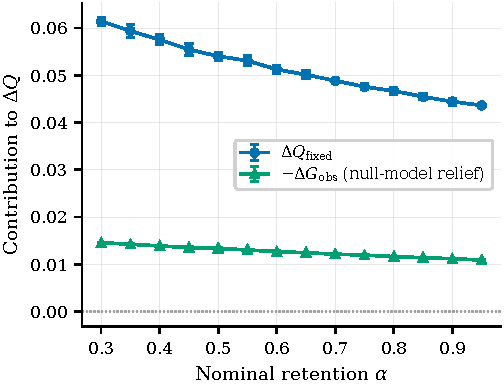
\includegraphics[width=0.85\linewidth]{figures/cit-HepTh_figure_B_decomposition_no_alpha1.pdf}
  \caption{Modularity decomposition under DSpar sparsification on \texttt{cit-HepTh}: $\Delta Q_{\mathrm{fixed}}$ alongside the null-model contribution $-\Delta G_{\mathrm{obs}}$ across sparsification levels; the remainder is $\Delta F_{\mathrm{obs}}$ (Table~\ref{tab:exp1_2_decomposition}).}
  \label{fig:decomposition_cit_hepth}
\end{figure}

\paragraph{What is \emph{not} shown.}
These measurements verify the mechanism of Section~\ref{sec:theory}: degree-biased sampling shifts edge composition and null-model mass exactly as predicted.
They do not show that community detection improved.
Both $\Delta Q$ columns compare modularity \emph{across different graphs} (the fixed partition scored on $G$ versus on the sparsified $G'$); presented without controls, such measurements read as evidence of improvement, and Section~\ref{sec:artifacts} demonstrates why that reading fails.

\subsection{Configuration-Model Controls}
\label{sec:mech-null}

If $\delta > 0$ and $\Delta Q_{\mathrm{fixed}} > 0$ reflected community structure, they should weaken or vanish on graphs whose communities have been destroyed.
We test this directly: each network is degree-preservingly rewired ($10m$ edge swaps), Leiden is run on the rewired graph to obtain its fixed partition, and the identical pipeline is applied.
Rewiring collapses modularity itself (base $Q$ drops from $0.42$--$0.93$ to $0.11$--$0.49$, the residue a maximizer extracts from degree noise~\cite{guimera2004modularity}), so any surviving signal is attributable to the degree sequence alone.

\begin{table*}[t]
\centering
\setlength{\tabcolsep}{3pt}
\caption{Configuration-model null control. For each network the degree sequence is preserved
exactly by double-edge swaps ($10m$ swaps), which destroys community structure; the sparsifier
(DSpar, \texttt{method="paper"}, nominal $\alpha=0.8$) and the fixed-partition decomposition are
then applied identically to both arms. The rewired null reproduces \emph{both} signals the draft
read as evidence of community structure: $\delta>0$ in 17/17 nulls and $\Delta Q_{\mathrm{fixed}}>0$
in 17/17 nulls, with $\Delta Q_{\mathrm{fixed}}(\mathrm{null})\ge\Delta Q_{\mathrm{fixed}}(\mathrm{real})$
in 15/17 networks (median ratio $1.24$) and $\delta(\mathrm{null})\ge\delta(\mathrm{real})$ in 16/17.
facebook-combined is the only network with $\delta<0$ on the real graph (bold), yet its null is still
$\delta>0$. Realized retention is $m'/m$: the with-replacement \texttt{paper} sampler retains far
fewer distinct edges than the nominal $\alpha$ (see Table~\ref{tab:sampler_audit}).
Real arm: 1 Leiden partition $\times$ 3 sparsification seeds; null arm: 2 rewire seeds $\times$
2 sparsification seeds (1 $\times$ 2 for cit-Patents and wiki-topcats). Standard deviations over
replicates are shown for $\Delta Q_{\mathrm{fixed}}$; for the remaining columns they are
$\le 0.002$ ($Q_{\mathrm{fixed}}^{\mathrm{base}}$), $\le 0.004$ ($\delta$), $\le 0.175$ ($\mathrm{hb}$) and
$\le 0.004$ (retention).}
\label{tab:null_control}
\footnotesize
\begin{tabular}{lrrrrrrrrrrr}
\toprule
 & & \multicolumn{2}{c}{$Q_{\mathrm{fixed}}^{\mathrm{base}}$} & \multicolumn{2}{c}{$\delta$}
 & \multicolumn{2}{c}{$\mathrm{hb}$} & \multicolumn{2}{c}{$\Delta Q_{\mathrm{fixed}}$}
 & \multicolumn{2}{c}{realized ret.} \\
\cmidrule(lr){3-4}\cmidrule(lr){5-6}\cmidrule(lr){7-8}\cmidrule(lr){9-10}\cmidrule(lr){11-12}
Network & $m$ & real & null & real & null & real & null & real & null & real & null \\
\midrule
email-Eu-core & 16,064 & 0.4159 & 0.1274 & +0.034 & +0.041 & 2.113 & 1.404 & +0.0819 $\pm$ 0.0044 & +0.0350 $\pm$ 0.0032 & 0.444 & 0.447 \\
wiki-Vote & 100,736 & 0.4240 & 0.1260 & +0.051 & +0.101 & 1.902 & 1.689 & +0.0711 $\pm$ 0.0012 & +0.0843 $\pm$ 0.0012 & 0.332 & 0.333 \\
ca-GrQc & 13,422 & 0.8514 & 0.3768 & +0.087 & +0.189 & 0.478 & 1.758 & +0.0176 $\pm$ 0.0058 & +0.0991 $\pm$ 0.0031 & 0.452 & 0.474 \\
ca-HepTh & 24,806 & 0.7619 & 0.4129 & +0.174 & +0.215 & 1.581 & 1.929 & +0.0523 $\pm$ 0.0022 & +0.0941 $\pm$ 0.0016 & 0.477 & 0.483 \\
facebook-combined & 88,234 & 0.8355 & 0.1146 & \textbf{$-$0.001} & +0.017 & 2.681 & 1.391 & +0.0256 $\pm$ 0.0013 & +0.0270 $\pm$ 0.0005 & 0.437 & 0.460 \\
ca-CondMat & 91,286 & 0.7312 & 0.3119 & +0.113 & +0.102 & 2.490 & 1.493 & +0.0606 $\pm$ 0.0006 & +0.0667 $\pm$ 0.0012 & 0.472 & 0.482 \\
ca-HepPh & 117,619 & 0.6512 & 0.1571 & +0.021 & +0.094 & 0.501 & 1.872 & +0.0864 $\pm$ 0.0016 & +0.0917 $\pm$ 0.0016 & 0.340 & 0.383 \\
ca-AstroPh & 196,972 & 0.6343 & 0.1676 & +0.033 & +0.041 & 1.496 & 1.294 & +0.0393 $\pm$ 0.0008 & +0.0489 $\pm$ 0.0011 & 0.417 & 0.436 \\
email-Enron & 180,811 & 0.6124 & 0.2420 & +0.150 & +0.240 & 2.974 & 4.472 & +0.1422 $\pm$ 0.0004 & +0.1562 $\pm$ 0.0013 & 0.389 & 0.394 \\
cit-HepTh & 352,021 & 0.6567 & 0.1583 & +0.026 & +0.032 & 2.173 & 1.778 & +0.0461 $\pm$ 0.0002 & +0.0376 $\pm$ 0.0006 & 0.434 & 0.453 \\
cit-HepPh & 420,784 & 0.7314 & 0.1675 & +0.011 & +0.026 & 1.358 & 1.300 & +0.0126 $\pm$ 0.0003 & +0.0319 $\pm$ 0.0004 & 0.459 & 0.468 \\
com-Amazon & 925,872 & 0.9296 & 0.4235 & +0.010 & +0.139 & 1.042 & 2.139 & +0.0000 $\pm$ 0.0001 & +0.0586 $\pm$ 0.0005 & 0.515 & 0.512 \\
com-DBLP & 1,049,866 & 0.8271 & 0.3647 & +0.147 & +0.197 & 1.583 & 2.308 & +0.0437 $\pm$ 0.0002 & +0.0980 $\pm$ 0.0005 & 0.469 & 0.475 \\
com-Youtube & 2,987,624 & 0.7188 & 0.4024 & +0.246 & +0.552 & 3.996 & 14.066 & +0.0959 $\pm$ 0.0002 & +0.2633 $\pm$ 0.0002 & 0.410 & 0.408 \\
wiki-Talk & 4,656,682 & 0.5995 & 0.4878 & +0.513 & +0.831 & 10.477 & 105.630 & +0.2020 $\pm$ 0.0002 & +0.3529 $\pm$ 0.0001 & 0.455 & 0.415 \\
cit-Patents & 16,511,740 & 0.8268 & 0.2962 & +0.038 & +0.166 & 0.723 & 1.940 & +0.0047 $\pm$ 0.0001 & +0.0768 $\pm$ 0.0000 & 0.461 & 0.467 \\
wiki-topcats & 25,444,207 & 0.6452 & 0.1412 & +0.023 & +0.029 & 5.076 & 6.920 & +0.0484 $\pm$ 0.0001 & +0.0538 $\pm$ 0.0000 & 0.447 & 0.435 \\
\bottomrule
\end{tabular}
\end{table*}


Table~\ref{tab:null_control} shows the result: the null reproduces \emph{both} signals on every network.
DSpar separation is positive on $17/17$ rewired graphs and \emph{exceeds} the real graph's value on $16/17$; fixed-partition modularity gains are positive on $17/17$ and exceed the real graph's on $15/17$, with median ratio $1.24$.
The sharpest cases are those where the real graph's signal is weakest: \texttt{com-Amazon} (real $\Delta Q_{\mathrm{fixed}} = 1.5\times10^{-5}$, null $0.059$), \texttt{cit-Patents} ($0.005$ vs.\ $0.077$), and \texttt{facebook-combined}, whose real $\delta$ is \emph{negative} ($-0.0014$) while its null is positive.
Hub-bridging behaves identically: the ratio exceeds one on $17/17$ nulls, reaching $105.6$ on rewired \texttt{wiki-Talk}, while on the real graphs it is erratic ($0.48$--$10.5$), falling below one on three networks.

A degree-biased sampler preferentially thins hub-incident edges, raising fixed-partition modularity for \emph{any} partition on \emph{any} degree-heterogeneous graph; positive $\delta$, positive $\Delta Q_{\mathrm{fixed}}$, and hub-bridging above one are thus properties of heavy-tailed degree sequences interacting with modularity optimization, and their sign carries no information about community structure.
Consequently, correlations between $\delta$ and $\Delta Q_{\mathrm{fixed}}$ across networks (however strong) validate only the arithmetic of Theorems~\ref{thm:ratio}--\ref{thm:sparsification}, not any claim about community structure: the two quantities are linked mechanically through the same score distribution.

The control also yields a sharper observation: the signals are not merely reproduced but systematically \emph{stronger} on the rewired graphs ($\delta$ larger on $16/17$, $\Delta Q_{\mathrm{fixed}}$ larger on $15/17$). Real community structure evidently suppresses both quantities relative to pure degree noise, so the pair $(\delta, \delta_{\mathrm{null}})$ does separate real networks from their configuration models, with the opposite sign from the naive reading; why real structure has this effect is an open question (Section~\ref{sec:discussion}).

Uniform random sparsification provides the complementary control: its fixed-partition change is zero within $\pm 0.001$ on real and rewired graphs alike, even at DSpar's realized retention, where DSpar registers $+0.04$ to $+0.14$; in expectation, unbiased edge deletion scales both modularity terms equally. The fixed-partition inflation therefore requires degree-\emph{biased} removal specifically, while the cross-graph inflation of Section~\ref{sec:artifact-modularity} requires only edge removal. The two artifacts are distinct mechanisms, and the two controls (configuration-model null; fixed-objective scoring) detect different failure modes: neither substitutes for the other.

\subsection{Partition Provenance}
\label{sec:mech-provenance}

A second confound concerns \emph{which partition} $\delta$ is measured against.
On standard LFR benchmarks~\cite{lancichinetti2008benchmark} ($n = 10^4$, $\mu \in \{0.1,\dots,0.5\}$), $\delta$ is negative with respect to the \emph{planted} partition at every mixing level ($-0.003$ to $-0.010$).
Measured instead against a \emph{Leiden} partition of the same graph, $\delta$ shifts systematically positive at every $\mu$, and the shift grows exactly as Leiden departs from the planted truth (at $\mu = 0.5$: NMI to planted $0.67$, planted communities merged from $236$ to $48$, shift $+0.0032$).
The shift does not flip the sign on LFR, whose degree distribution is nearly homogeneous under standard parameterizations (coefficient of variation $\approx 0.4$, versus $1.0$--$26$ on the real networks in our suite), but on heavy-tailed real networks it can: on \texttt{com-Amazon}, $\delta = -0.004$ against the ground-truth communities and $+0.01$ against the Leiden partition of the same graph.
Positive DSpar separation, as reported in practice, is therefore a joint property of heavy-tailed degrees \emph{and} of partitions produced by modularity optimization; comparisons between $\delta$ values measured against planted partitions (synthetic benchmarks) and detected partitions (real networks) are not like-for-like.

\subsection{Controlled Hub-Bridging in Synthetic Benchmarks}
\label{sec:mech-lfr}

Finally, we include a controlled synthetic experiment, stated with the caveats above.
Standard LFR graphs exhibit hub-bridging ratios below one and negative $\delta$ (planted partition), and sparsification lowers fixed-partition modularity ($\Delta Q_{\mathrm{fixed}} = -0.009$ at $\mu = 0.3$, $n = 10^4$, nominal $\alpha = 0.8$).
We then rewire $70\%$ of inter-community edges, re-attaching endpoints within their communities with probability proportional to $d^{\,h}$, where $h \ge 1$ controls the strength of degree preference; this preserves the number of inter-community edges (hence $\mu$) while inducing controllable hub-bridging.
At $h = 4$ the hub-bridging ratio reaches $\approx 15.9$, $\delta$ turns positive ($+0.051$), and fixed-partition modularity change turns strongly positive ($+0.106$), with $\Delta Q_{\mathrm{fixed}}$ tightly coupled to the hub-bridging ratio across all configurations (Figure~\ref{fig:lfr_dq_vs_hubratio}).

\begin{figure}[t]
  \centering
  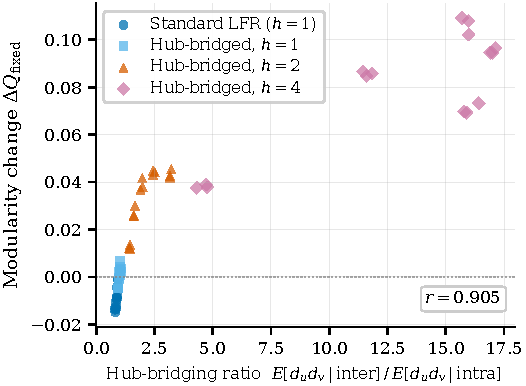
\includegraphics[width=0.85\linewidth]{figures/plot3_dQ_vs_hub_ratio_n10000_r0.8.pdf}
\caption{Fixed-partition modularity change under DSpar as a function of induced hub-bridging on LFR graphs ($n = 10^4$, nominal $\alpha = 0.8$, planted partitions). The controlled rewiring operator ($h$: endpoint choice $\propto d^{\,h}$) restores the coupling between hub-bridging, $\delta$, and $\Delta Q_{\mathrm{fixed}}$.}
  \label{fig:lfr_dq_vs_hubratio}
\end{figure}

Read through the lens of \S\ref{sec:mech-null}, this experiment demonstrates \emph{controllability of the mechanism}: degree--community coupling is the knob that turns fixed-partition gains on and off. It makes no statement about detection quality.
It also identifies a genuine limitation of LFR as a benchmark for sparsification studies: standard LFR lacks both the heavy-tailed degree profile and the degree--community coupling that real networks and their configuration models exhibit.


\section{Three Evaluation Artifacts}
\label{sec:artifacts}

We now analyze the three evaluation designs by which sparsification appears to improve community detection, and pair each with the control that exposes it.

\subsection{Artifact I: Modularity Is Not Comparable Across Graphs}
\label{sec:artifact-modularity}

The quantities $\Delta Q_{\mathrm{fixed}}$ and $\Delta Q_{\mathrm{Leiden}}^{\mathrm{(sp)}}$ of Section~\ref{sec:mechanism} compare a partition's modularity on the sparsified graph against a (possibly different) partition's modularity on the original graph.
Modularity, however, is defined relative to a graph's own configuration null model; changing the edge set changes the yardstick.
Sparser graphs support higher modularity for combinatorial reasons unrelated to community structure~\cite{guimera2004modularity}, and altering $m$ shifts the resolution at which modularity operates~\cite{fortunato2007resolution}.
A quality claim requires a fixed objective: \emph{score every partition on the original graph}.

\begin{table*}[t]
\centering
\setlength{\tabcolsep}{5pt}
\caption{Artifact I --- cross-graph modularity. $Q_{\mathrm{sparse}}$ is the modularity of the
partition found on the sparsified graph, \emph{scored on that sparsified graph}; $Q_{\mathrm{orig}}$
is the same partition scored on the original graph; the transfer loss is
$Q_{\mathrm{base}}-Q_{\mathrm{orig}}$, the unsparsified baseline minus the transferred partition's score. It is positive for all 15 datasets at both $\alpha$ values,
i.e.\ the headline ``modularity gain'' of the sparsify-then-cluster pipeline is an artifact of
comparing scores computed on two different graphs. $Q_{\mathrm{final}}$ is Leiden seeded with the
sparse-graph partition and run on the original graph, and $\Delta Q$ is that value minus the
unsparsified baseline; the honest gain is $\le 0.008$ everywhere.
Realized retention is $m'/m$ (\texttt{paper} sampler, with replacement), not the nominal $\alpha$.
The $\alpha=1.0$ rows of the source file are \emph{not} baselines --- the sampler still ran
(realized retention $0.350$--$0.589$) --- and are excluded here; the unsparsified reference is the
run's own $Q_{\mathrm{base}}$, embedded in $\Delta Q$.
5 seeds per cell; $\pm$ is the standard deviation over seeds ($\Delta Q$ and the transfer loss are
reported without one, as the source file stores no standard deviation for them).}
\label{tab:transfer_loss}
\footnotesize
\begin{tabular}{llrrrrrr}
\toprule
Dataset & $\alpha$ & realized ret. & $Q_{\mathrm{sparse}}$ & $Q_{\mathrm{orig}}$
 & transfer loss & $Q_{\mathrm{final}}$ & $\Delta Q$ \\
\midrule
\multirow{2}{*}{ca-AstroPh} & 0.8 & 0.417 & 0.6902 $\pm$ 0.0011 & 0.6019 $\pm$ 0.0033 & 0.0334 & 0.6360 $\pm$ 0.0015 & +0.0006 \\
 & 0.9 & 0.446 & 0.6853 $\pm$ 0.0014 & 0.6047 $\pm$ 0.0035 & 0.0307 & 0.6358 $\pm$ 0.0012 & +0.0004 \\
\addlinespace[2pt]
\multirow{2}{*}{ca-CondMat} & 0.8 & 0.473 & 0.8310 $\pm$ 0.0004 & 0.6597 $\pm$ 0.0017 & 0.0752 & 0.7348 $\pm$ 0.0013 & $-$0.0000 \\
 & 0.9 & 0.506 & 0.8234 $\pm$ 0.0006 & 0.6721 $\pm$ 0.0023 & 0.0628 & 0.7350 $\pm$ 0.0014 & +0.0001 \\
\addlinespace[2pt]
\multirow{2}{*}{ca-GrQc} & 0.8 & 0.456 & 0.9002 $\pm$ 0.0003 & 0.7797 $\pm$ 0.0018 & 0.0722 & 0.8517 $\pm$ 0.0005 & $-$0.0002 \\
 & 0.9 & 0.485 & 0.8947 $\pm$ 0.0006 & 0.7924 $\pm$ 0.0024 & 0.0595 & 0.8518 $\pm$ 0.0005 & $-$0.0001 \\
\addlinespace[2pt]
\multirow{2}{*}{ca-HepPh} & 0.8 & 0.339 & 0.7634 $\pm$ 0.0009 & 0.6209 $\pm$ 0.0056 & 0.0408 & 0.6610 $\pm$ 0.0008 & $-$0.0006 \\
 & 0.9 & 0.360 & 0.7605 $\pm$ 0.0010 & 0.6279 $\pm$ 0.0027 & 0.0338 & 0.6615 $\pm$ 0.0009 & $-$0.0001 \\
\addlinespace[2pt]
\multirow{2}{*}{ca-HepTh} & 0.8 & 0.475 & 0.8825 $\pm$ 0.0005 & 0.6324 $\pm$ 0.0031 & 0.1320 & 0.7645 $\pm$ 0.0008 & +0.0002 \\
 & 0.9 & 0.507 & 0.8681 $\pm$ 0.0005 & 0.6532 $\pm$ 0.0031 & 0.1111 & 0.7644 $\pm$ 0.0009 & +0.0001 \\
\addlinespace[2pt]
\multirow{2}{*}{cit-HepPh} & 0.8 & 0.460 & 0.7512 $\pm$ 0.0020 & 0.7220 $\pm$ 0.0039 & 0.0123 & 0.7349 $\pm$ 0.0009 & +0.0007 \\
 & 0.9 & 0.493 & 0.7486 $\pm$ 0.0022 & 0.7222 $\pm$ 0.0032 & 0.0121 & 0.7355 $\pm$ 0.0010 & +0.0012 \\
\addlinespace[2pt]
\multirow{2}{*}{cit-HepTh} & 0.8 & 0.433 & 0.7178 $\pm$ 0.0013 & 0.6486 $\pm$ 0.0027 & 0.0143 & 0.6629 $\pm$ 0.0026 & +0.0000 \\
 & 0.9 & 0.465 & 0.7148 $\pm$ 0.0015 & 0.6509 $\pm$ 0.0018 & 0.0120 & 0.6624 $\pm$ 0.0026 & $-$0.0005 \\
\addlinespace[2pt]
\multirow{2}{*}{com-Amazon} & 0.8 & 0.516 & 0.9519 $\pm$ 0.0001 & 0.8502 $\pm$ 0.0004 & 0.0815 & 0.9324 $\pm$ 0.0001 & +0.0007 \\
 & 0.9 & 0.554 & 0.9480 $\pm$ 0.0001 & 0.8728 $\pm$ 0.0004 & 0.0589 & 0.9325 $\pm$ 0.0001 & +0.0008 \\
\addlinespace[2pt]
\multirow{2}{*}{com-DBLP} & 0.8 & 0.469 & 0.9090 $\pm$ 0.0003 & 0.7429 $\pm$ 0.0018 & 0.0879 & 0.8338 $\pm$ 0.0004 & +0.0031 \\
 & 0.9 & 0.501 & 0.9024 $\pm$ 0.0002 & 0.7599 $\pm$ 0.0011 & 0.0709 & 0.8337 $\pm$ 0.0004 & +0.0029 \\
\addlinespace[2pt]
\multirow{2}{*}{com-Youtube} & 0.8 & 0.410 & 0.8901 $\pm$ 0.0005 & 0.5483 $\pm$ 0.0043 & 0.1801 & 0.7281 $\pm$ 0.0002 & $-$0.0003 \\
 & 0.9 & 0.434 & 0.8789 $\pm$ 0.0002 & 0.5811 $\pm$ 0.0019 & 0.1472 & 0.7281 $\pm$ 0.0003 & $-$0.0003 \\
\addlinespace[2pt]
\multirow{2}{*}{email-Enron} & 0.8 & 0.389 & 0.7942 $\pm$ 0.0006 & 0.5683 $\pm$ 0.0026 & 0.0464 & 0.6219 $\pm$ 0.0021 & +0.0072 \\
 & 0.9 & 0.413 & 0.7860 $\pm$ 0.0009 & 0.5739 $\pm$ 0.0031 & 0.0408 & 0.6225 $\pm$ 0.0017 & +0.0078 \\
\addlinespace[2pt]
\multirow{2}{*}{facebook-combined} & 0.8 & 0.436 & 0.8625 $\pm$ 0.0003 & 0.8314 $\pm$ 0.0009 & 0.0043 & 0.8357 $\pm$ 0.0001 & +0.0000 \\
 & 0.9 & 0.467 & 0.8624 $\pm$ 0.0003 & 0.8313 $\pm$ 0.0009 & 0.0044 & 0.8355 $\pm$ 0.0005 & $-$0.0002 \\
\addlinespace[2pt]
\multirow{2}{*}{soc-Epinions1} & 0.8 & 0.317 & 0.6931 $\pm$ 0.0021 & 0.3225 $\pm$ 0.0115 & 0.1283 & 0.4500 $\pm$ 0.0033 & $-$0.0008 \\
 & 0.9 & 0.334 & 0.6783 $\pm$ 0.0019 & 0.3439 $\pm$ 0.0114 & 0.1068 & 0.4514 $\pm$ 0.0034 & +0.0006 \\
\addlinespace[2pt]
\multirow{2}{*}{wiki-Talk} & 0.8 & 0.455 & 0.8974 $\pm$ 0.0000 & 0.4169 $\pm$ 0.0004 & 0.1852 & 0.6027 $\pm$ 0.0001 & +0.0006 \\
 & 0.9 & 0.483 & 0.8860 $\pm$ 0.0000 & 0.4373 $\pm$ 0.0004 & 0.1648 & 0.6028 $\pm$ 0.0002 & +0.0007 \\
\addlinespace[2pt]
\multirow{2}{*}{wiki-Vote} & 0.8 & 0.333 & 0.5119 $\pm$ 0.0055 & 0.4004 $\pm$ 0.0065 & 0.0244 & 0.4250 $\pm$ 0.0033 & +0.0002 \\
 & 0.9 & 0.357 & 0.5104 $\pm$ 0.0039 & 0.4081 $\pm$ 0.0027 & 0.0168 & 0.4255 $\pm$ 0.0034 & +0.0007 \\
\bottomrule
\end{tabular}
\end{table*}


Table~\ref{tab:transfer_loss} applies this control across 15 networks.
We define the \emph{transfer loss} as $Q_{\mathrm{base}} - Q_{G}(P_\alpha)$: the unsparsified baseline minus the transferred partition's modularity on the original graph.
The partition obtained by running Leiden on the sparsified graph scores far above baseline on the sparsified graph (e.g., \texttt{wiki-Talk}: $0.897$ vs.\ $0.602$), and \emph{below} baseline once evaluated on the original graph ($0.417$), a transfer loss of $0.185$.
Transfer loss is positive on all 15 networks at every tested retention: what appears as a gain of $+0.01$ to $+0.30$ on the sparsified graph is, on the fixed objective, a loss of $0.004$ to $0.19$; the sign of the conclusion reverses on every dataset.
Refining the transferred partition on the original graph (column $Q_{\mathrm{final}}$) recovers the baseline almost exactly, leaving residuals of $-0.001$ to $+0.008$; Section~\ref{sec:boundary} examines when those residuals are genuine.
The artifact is not specific to DSpar: uniform random edge deletion, a sampler with no structural intelligence at all, reproduces the same sign flip on every configuration we tested (three networks, two retention levels: apparent gains of $+0.001$ to $+0.011$ on the sparsified graph, losses of $0.006$--$0.025$ on the original). Cross-graph inflation is a property of the scoring convention, not of any particular sparsifier.

\subsection{Artifact II: Partition Granularity}
\label{sec:artifact-granularity}

Sparsification fragments graphs, and detection on fragmented graphs returns finer partitions.
Against small reference communities, as ground-truth sets in common benchmarks are, finer partitions score better on popular agreement measures for reasons unrelated to the preprocessing: uncorrected NMI is biased toward many clusters~\cite{vinh2010information}, and set-matching scores such as average $F_1$ reward granularity against small targets, since splitting clusters moves candidate sets toward the size of the small reference communities.
The control is to grant the \emph{baseline} the same granularity: run the same algorithm on the \emph{unsparsified} graph with the resolution parameter tuned to match the sparsified pipeline's cluster count.

\paragraph{At scale.}
On SNAP networks with functional ground truth (top-5000 communities; median size 7--8 nodes), the with-replacement DSpar pipeline at nominal $\alpha=0.8$ appears to help on two of three datasets (average $F_1$, mean of both matching directions: \texttt{com-Amazon} $0.211 \to 0.285$; \texttt{com-Youtube} $0.010 \to 0.050$; \texttt{com-DBLP} $0.146 \to 0.100$), while inflating cluster counts $21$--$42\times$.
The resolution-matched control, using every edge, beats the sparsified pipeline everywhere, by wide margins: $0.404$ on \texttt{com-Amazon}, $0.293$ on \texttt{com-DBLP}, $0.129$ on \texttt{com-Youtube}.
The apparent recovery gain is obtainable, doubled, without discarding a single edge; the discarded edges are pure loss.
Mild pruning via the clipped no-replacement sampler at nominal $0.9$ (true retention $0.52$--$0.76$) moves recovery by $-0.037$ to $+0.001$, indistinguishable from zero.

\paragraph{On classical labeled graphs.}
\begin{table*}[t]
\centering
\setlength{\tabcolsep}{5pt}
\caption{Artifact II --- granularity. Ground-truth recovery on the five small benchmark graphs,
10 seeds per cell, mean $\pm$ standard deviation. \emph{baseline} is Leiden on the original graph;
\emph{DSpar \texttt{paper}} is the draft's pipeline (with-replacement sampler, nominal $\alpha=0.8$,
realized retention $0.44$--$0.55$); the \emph{resolution-matched control} applies no sparsification
at all and instead tunes the RBConfiguration resolution $\gamma$ on the original graph until the
cluster count matches the DSpar run; \emph{DSpar calibrated} uses the $\lambda$-bisection sampler
with $\mathbb{E}[\text{retention}]=0.9$ exactly. AMI is the chance-corrected primary metric; NMI is
the draft's metric and is inflated by the finer partitions sparsification produces. The only
positive cell in the draft (email-Eu-core) is reproduced and exceeded by the resolution-matched
control at 100\% of the edges ($\Delta$AMI $+0.014$ vs $+0.007$), so the score against a
granularity-matched baseline is 0/5.}
\label{tab:gt_recheck}
\footnotesize
\begin{tabular}{llrrrrrr}
\toprule
Dataset & Condition & true ret. & $\gamma$ & \#clusters & AMI & ARI & NMI \\
\midrule
\multirow{4}{*}{Karate} & baseline (no sparsification) & 1.000 & 1.000 & 4.0 $\pm$ 0.0 & 0.557 $\pm$ 0.028 & 0.457 $\pm$ 0.022 & 0.579 $\pm$ 0.027 \\
 & DSpar \texttt{paper}, $\alpha=0.8$ & 0.541 & 1.000 & 7.3 $\pm$ 1.7 & 0.366 $\pm$ 0.059 & 0.294 $\pm$ 0.073 & 0.429 $\pm$ 0.050 \\
 & resolution-matched control & 1.000 & 2.000 & 7.3 $\pm$ 0.5 & 0.392 $\pm$ 0.005 & 0.239 $\pm$ 0.009 & 0.445 $\pm$ 0.003 \\
 & DSpar calibrated, $\alpha=0.9$ & 0.887 & 1.000 & 4.0 $\pm$ 0.0 & 0.492 $\pm$ 0.038 & 0.416 $\pm$ 0.031 & 0.517 $\pm$ 0.036 \\
\addlinespace[2pt]
\multirow{4}{*}{Dolphins$^{\dagger}$} & baseline (no sparsification) & 1.000 & 1.000 & 5.0 $\pm$ 0.4 & 0.270 $\pm$ 0.029 & 0.246 $\pm$ 0.033 & 0.293 $\pm$ 0.027 \\
 & DSpar \texttt{paper}, $\alpha=0.8$ & 0.520 & 1.000 & 9.7 $\pm$ 1.2 & 0.216 $\pm$ 0.045 & 0.132 $\pm$ 0.029 & 0.264 $\pm$ 0.039 \\
 & resolution-matched control & 1.000 & 2.300 & 10.3 $\pm$ 0.9 & 0.223 $\pm$ 0.018 & 0.125 $\pm$ 0.010 & 0.270 $\pm$ 0.014 \\
 & DSpar calibrated, $\alpha=0.9$ & 0.892 & 1.000 & 4.9 $\pm$ 0.5 & 0.261 $\pm$ 0.021 & 0.195 $\pm$ 0.047 & 0.284 $\pm$ 0.019 \\
\addlinespace[2pt]
\multirow{4}{*}{Football} & baseline (no sparsification) & 1.000 & 1.000 & 9.7 $\pm$ 0.5 & 0.849 $\pm$ 0.018 & 0.779 $\pm$ 0.047 & 0.880 $\pm$ 0.016 \\
 & DSpar \texttt{paper}, $\alpha=0.8$ & 0.549 & 1.000 & 9.2 $\pm$ 0.9 & 0.812 $\pm$ 0.032 & 0.737 $\pm$ 0.059 & 0.849 $\pm$ 0.028 \\
 & resolution-matched control & 1.000 & 1.000 & 9.7 $\pm$ 0.5 & 0.849 $\pm$ 0.018 & 0.779 $\pm$ 0.047 & 0.880 $\pm$ 0.016 \\
 & DSpar calibrated, $\alpha=0.9$ & 0.899 & 1.000 & 8.9 $\pm$ 0.3 & 0.816 $\pm$ 0.013 & 0.702 $\pm$ 0.027 & 0.852 $\pm$ 0.011 \\
\addlinespace[2pt]
\multirow{4}{*}{Polbooks} & baseline (no sparsification) & 1.000 & 1.000 & 4.7 $\pm$ 0.5 & 0.535 $\pm$ 0.026 & 0.625 $\pm$ 0.061 & 0.551 $\pm$ 0.024 \\
 & DSpar \texttt{paper}, $\alpha=0.8$ & 0.527 & 1.000 & 6.8 $\pm$ 0.7 & 0.413 $\pm$ 0.043 & 0.341 $\pm$ 0.069 & 0.439 $\pm$ 0.041 \\
 & resolution-matched control & 1.000 & 1.500 & 6.8 $\pm$ 0.6 & 0.431 $\pm$ 0.012 & 0.333 $\pm$ 0.021 & 0.456 $\pm$ 0.010 \\
 & DSpar calibrated, $\alpha=0.9$ & 0.900 & 1.000 & 5.2 $\pm$ 0.7 & 0.475 $\pm$ 0.028 & 0.490 $\pm$ 0.088 & 0.494 $\pm$ 0.025 \\
\addlinespace[2pt]
\multirow{4}{*}{email-Eu-core} & baseline (no sparsification) & 1.000 & 1.000 & 7.7 $\pm$ 0.5 & 0.558 $\pm$ 0.010 & 0.323 $\pm$ 0.021 & 0.583 $\pm$ 0.011 \\
 & DSpar \texttt{paper}, $\alpha=0.8$ & 0.443 & 1.000 & 8.6 $\pm$ 0.5 & 0.565 $\pm$ 0.014 & 0.360 $\pm$ 0.026 & 0.592 $\pm$ 0.013 \\
 & resolution-matched control & 1.000 & 1.075 & 8.6 $\pm$ 0.9 & 0.571 $\pm$ 0.017 & 0.361 $\pm$ 0.043 & 0.598 $\pm$ 0.018 \\
 & DSpar calibrated, $\alpha=0.9$ & 0.900 & 1.000 & 7.3 $\pm$ 0.6 & 0.549 $\pm$ 0.024 & 0.298 $\pm$ 0.037 & 0.573 $\pm$ 0.024 \\
\bottomrule
\end{tabular}

\vspace{2pt}
{\footnotesize\raggedright $^{\dagger}$Dolphins has no canonical ground-truth partition; the labels
used here are a surrogate two-group split obtained by Kernighan--Lin bisection, so its recovery
scores measure agreement with a heuristic cut, not with metadata.\par}
\end{table*}

Table~\ref{tab:gt_recheck} repeats the analysis on five classical labeled datasets, adding chance-corrected AMI~\cite{vinh2010information} as the primary measure.
Four of the five datasets are negative under every metric, and become \emph{more} negative under AMI (e.g., Karate $\Delta\mathrm{AMI} = -0.19$).
The one apparent positive, \texttt{email-Eu-core}, does not survive: its $\Delta\mathrm{AMI} = +0.007 \pm 0.019$ is statistically indistinguishable from zero, and the resolution-matched control exceeds the sparsified pipeline on all three metrics.
Under calibrated true-$0.9$ retention the effect is negative even nominally; the residual positive depended on the with-replacement sampler discarding $56\%$ of edges, not on the degree scores.
We note additionally that reference labels are themselves imperfect proxies for structural communities~\cite{peel2017ground, hric2014community}, and that one dataset's conventional labels proved on inspection to be an algorithmic surrogate rather than observed metadata (Table~\ref{tab:gt_recheck}, footnote).

\subsection{Artifact III: Unmatched Computation}
\label{sec:artifact-compute}

A sparsify--cluster--refine pipeline performs more optimization than the single baseline run it is typically compared against.
The control is to grant the baseline equal wall-clock time, spent on independent restarts, and compare against the best.
In our measurements the pipeline costs $1.5$--$2.0\times$ a single Leiden run (sparsification itself is $2$--$10\%$ of the total), so the matched baseline is best-of-two restarts; best-of-two costs $2.0\times$, at or slightly above the pipeline, and the slack favors the baseline (conservative for reported gains, mildly anti-conservative for reported losses).
The correction is not cosmetic: on \texttt{wiki-Vote}, the seeded pipeline beats the \emph{mean} baseline in six of eight configurations and loses to the runtime-matched baseline in all eight.
Comparisons against single-run means manufacture false positives whenever the optimizer's seed variance is nonzero.

\subsection{The Resulting Protocol}
\label{sec:protocol}

The three controls are general and cheap, and we suggest them as a minimal standard for any claim that preprocessing improves community detection:
\begin{enumerate}
    \item \textbf{Fixed objective}: evaluate all partitions on the \emph{original} graph (or an external reference), never on the preprocessed one.
    \item \textbf{Granularity matching}: give the baseline the preprocessing pipeline's cluster count via its resolution parameter; use chance-corrected agreement measures.
    \item \textbf{Compute matching}: give the baseline the pipeline's wall-clock budget via restarts, and compare best against best.
\end{enumerate}
To certify that a structural signal reflects community structure rather than degree structure, add the configuration-model null of Section~\ref{sec:mech-null}.


\section{The Boundary: Where Genuine Gains Exist}
\label{sec:boundary}

Having removed the artifacts, we ask what remains.
The one effect that survives all three controls is \emph{seeded refinement}: run Leiden on the sparsified graph, transfer the partition to the original graph, and continue optimizing there.
This uses sparsification not as a replacement for the graph but as a perturbation of the optimizer's search trajectory; the final quantity is modularity on the original graph, so Artifact~I does not arise, and we compare against runtime-matched restarts, so Artifact~III does not arise.

\subsection{Runtime-Matched Seeded Refinement}
\label{sec:boundary-seeded}

\begin{table*}[t]
\centering
\setlength{\tabcolsep}{5pt}
\caption{The boundary: runtime-matched seeded refinement, 15 networks, calibrated sampler at
$\alpha=0.9$ (realized retention $\approx 0.900$ by construction). $Q_{\mathrm{base}}$ is plain
Leiden on the original graph (5 seeds); $Q_{\mathrm{seeded}}$ is Leiden on the original graph seeded
with the sparse-graph partition (3 sparsification seeds); $Q_{\mathrm{matched}}$ is the best of the
plain-Leiden restarts affordable within the \emph{same} wall-clock budget as the full sparsify +
cluster + seed pipeline (2 restarts in all 15 cells). The honest outcome is
$y = Q_{\mathrm{seeded}} - Q_{\mathrm{matched}}$. Only 2/15 networks clear $y > 2\sigma_{\mathrm{base}}$
(starred, bold): email-Enron (robust across all tested configurations) and com-Youtube (a single-configuration candidate; see text). Genuine gains therefore exist, but they are rare and
small ($\le 0.009$).}
\label{tab:boundary}
\footnotesize
\begin{tabular}{lrrrrrrrc}
\toprule
Network & $n$ & $m$ & ret. & $Q_{\mathrm{base}}$ & $Q_{\mathrm{seeded}}$ & $Q_{\mathrm{matched}}$
 & $y$ & $y>2\sigma_{\mathrm{base}}$ \\
\midrule
email-Eu-core & 986 & 16,064 & 0.900 & 0.4160 $\pm$ 0.0004 & 0.4151 $\pm$ 0.0021 & 0.4174 & $-$0.0023 & no \\
wiki-Vote & 7,066 & 100,736 & 0.900 & 0.4244 $\pm$ 0.0025 & 0.4234 $\pm$ 0.0017 & 0.4294 & $-$0.0059 & no \\
ca-GrQc & 4,158 & 13,422 & 0.900 & 0.8506 $\pm$ 0.0010 & 0.8521 $\pm$ 0.0002 & 0.8517 & +0.0004 & no \\
ca-HepTh & 8,638 & 24,806 & 0.901 & 0.7614 $\pm$ 0.0009 & 0.7605 $\pm$ 0.0010 & 0.7621 & $-$0.0016 & no \\
facebook-combined & 4,039 & 88,234 & 0.900 & 0.8356 $\pm$ 0.0001 & 0.8356 $\pm$ 0.0003 & 0.8355 & +0.0001 & no \\
ca-CondMat & 21,363 & 91,286 & 0.900 & 0.7308 $\pm$ 0.0011 & 0.7312 $\pm$ 0.0005 & 0.7294 & +0.0018 & no \\
ca-HepPh & 11,204 & 117,619 & 0.900 & 0.6583 $\pm$ 0.0010 & 0.6599 $\pm$ 0.0016 & 0.6602 & $-$0.0003 & no \\
ca-AstroPh & 17,903 & 196,972 & 0.900 & 0.6308 $\pm$ 0.0027 & 0.6328 $\pm$ 0.0007 & 0.6316 & +0.0013 & no \\
\textbf{email-Enron} & 33,696 & 180,811 & 0.900 & 0.6071 $\pm$ 0.0019 & 0.6128 $\pm$ 0.0014 & 0.6051 & \textbf{+0.0077}$^{\ast}$ & yes \\
cit-HepTh & 27,400 & 352,021 & 0.900 & 0.6621 $\pm$ 0.0023 & 0.6611 $\pm$ 0.0018 & 0.6579 & +0.0032 & no \\
cit-HepPh & 34,401 & 420,784 & 0.900 & 0.7319 $\pm$ 0.0019 & 0.7335 $\pm$ 0.0014 & 0.7343 & $-$0.0008 & no \\
com-Amazon & 334,863 & 925,872 & 0.900 & 0.9294 $\pm$ 0.0003 & 0.9300 $\pm$ 0.0001 & 0.9296 & +0.0004 & no \\
com-DBLP & 317,080 & 1,049,866 & 0.900 & 0.8257 $\pm$ 0.0008 & 0.8281 $\pm$ 0.0002 & 0.8275 & +0.0006 & no \\
\textbf{com-Youtube} & 1,134,890 & 2,987,624 & 0.900 & 0.7245 $\pm$ 0.0034 & 0.7296 $\pm$ 0.0001 & 0.7209 & \textbf{+0.0086}$^{\ast}$ & yes \\
wiki-Talk & 2,388,953 & 4,656,682 & 0.900 & 0.6011 $\pm$ 0.0007 & 0.6015 $\pm$ 0.0003 & 0.6020 & $-$0.0006 & no \\
\bottomrule
\end{tabular}
\end{table*}


Table~\ref{tab:boundary} reports the outcome on 15 networks at calibrated retention $0.9$.
In the screening experiment, the seeded pipeline beats the runtime-matched baseline beyond twice the baseline's seed deviation on exactly \textbf{2 of 15} networks: \texttt{email-Enron} ($+0.0077$, $4.1$ baseline standard deviations) and \texttt{com-Youtube} ($+0.0086$, $2.5$); across 15 networks at a two-deviation screening threshold, roughly half a false positive is expected.
The \texttt{com-Youtube} margin as screened is inflated: its matched baseline is a single best-of-two realization that landed at the second percentile of the exact best-of-two distribution (all 45 pairs over ten baseline runs). A dedicated sweep (both samplers, $\alpha \in \{0.7, 0.8, 0.9, 0.95\}$, five seeds each) gives the corrected picture. Against the \emph{expected} best-of-two, the gain is confined to the calibrated sampler at $\alpha \ge 0.9$ and is small ($+0.0023$ at $\alpha = 0.9$, $+0.0031$ at $\alpha = 0.95$); the clipped sampler is negative in all four of its configurations, and aggressive calibrated sparsification ($\alpha = 0.7$) is strongly negative. The $\alpha = 0.95$ cell is nonetheless statistically solid: its seeded mean beats every one of the 45 matched best-of-two draws and all ten individual baseline runs (bootstrap $p < 10^{-4}$, surviving Bonferroni correction across the eight configurations), with across-seed spread $\pm 0.0004$. That the gain \emph{rises} as the sparsifier removes less marks it as a perturbation-of-the-optimizer effect rather than a sparsification benefit. We therefore report one substantial robust gain (\texttt{email-Enron}) and one small, regime-confined gain (\texttt{com-Youtube}).
The \texttt{email-Enron} result is robust across the sweep: against the runtime-matched best-of-two baseline it is positive in all eight configurations (both sampler variants, every retention level $0.7$--$0.95$; margins $+0.0007$ to $+0.0149$, the largest under the clipped no-replacement sampler at nominal $\alpha = 0.7$, true retention $0.45$), and against the stricter best-of-five baseline it is positive in seven of eight (margins up to $+0.0107$; the exception is calibrated $\alpha = 0.7$ at $-0.004$). That the margins grow under \emph{harsher} sparsification indicates the gain stems from aggressive hub-edge removal changing the optimizer's search space, not from mild denoising.
On \texttt{email-Enron} the raw transferred partition itself (before refinement) already exceeds baseline at true retention $\ge 0.8$, the only network in the suite where the transfer loss of Section~\ref{sec:artifact-modularity} changes sign.

\subsection{No Tested Statistic Predicts the Gains}
\label{sec:boundary-predictor}

\begin{table*}[t]
\centering
\setlength{\tabcolsep}{5pt}
\caption{No predictor of the genuine gain. Correlations between 14 candidate structural statistics
and the seeded-refinement outcome across the $n=15$ networks of Table~\ref{tab:boundary}.
$y = Q_{\mathrm{seeded}} - Q_{\mathrm{matched}}$ is the runtime-matched (honest) outcome;
$y_2 = Q_{\mathrm{seeded}} - Q_{\mathrm{base}}$ is the naive one. No predictor is significant for
$y$ at the $5\%$ level; the strongest is $n$ ($\rho=0.468$, $p=0.079$). Two cells reach nominal
significance against the \emph{naive} outcome only ($\mathrm{hb}$ excess, $p=0.026$; $n$, $p=0.044$), and
neither survives correction for the 28 tests reported here. $\delta^{\ast}$ --- the null-corrected
separation statistic --- is wrong-signed for both outcomes and is therefore retained as a diagnostic
only. With $n=15$, the $95\%$ CI of a single Pearson $r$ spans roughly $\pm 0.5$; see the wiki-Talk
case study in the text, where dropping one network moves $r(\mathrm{deg\ CV})$ from $0.69$ to $0.12$.}
\label{tab:predictors}
\footnotesize
\begin{tabular}{lrrrrrrrr}
\toprule
 & \multicolumn{4}{c}{$y$ (runtime-matched)} & \multicolumn{4}{c}{$y_2$ (naive)} \\
\cmidrule(lr){2-5}\cmidrule(lr){6-9}
Predictor & $\rho$ & $p$ & $r$ & $p$ & $\rho$ & $p$ & $r$ & $p$ \\
\midrule
$\delta$ (real graph) & +0.171 & 0.541 & +0.207 & 0.460 & +0.196 & 0.483 & +0.205 & 0.464 \\
$\delta^{\ast}=\delta_{\mathrm{real}}-\delta_{\mathrm{null}}$ & $-$0.075 & 0.791 & $-$0.360 & 0.188 & $-$0.386 & 0.156 & $-$0.398 & 0.142 \\
$\delta_{\mathrm{real}}/\delta_{\mathrm{null}}$ & +0.104 & 0.713 & +0.059 & 0.834 & $-$0.246 & 0.376 & $-$0.091 & 0.747 \\
$\Delta Q_{\mathrm{fixed}}^{\mathrm{real}}/\Delta Q_{\mathrm{fixed}}^{\mathrm{null}}$ & $-$0.089 & 0.752 & $-$0.166 & 0.556 & $-$0.429 & 0.111 & $-$0.341 & 0.214 \\
$\Delta Q_{\mathrm{fixed}}^{\mathrm{real}}-\Delta Q_{\mathrm{fixed}}^{\mathrm{null}}$ & $-$0.146 & 0.603 & $-$0.346 & 0.207 & $-$0.450 & 0.092 & $-$0.401 & 0.138 \\
$\mathrm{hb}$ (real graph) & +0.304 & 0.271 & +0.129 & 0.646 & $-$0.050 & 0.860 & +0.036 & 0.899 \\
$\mathrm{hb}_{\mathrm{real}}-\mathrm{hb}_{\mathrm{null}}$ & $-$0.211 & 0.451 & +0.038 & 0.893 & $-$0.571 & 0.026 & +0.040 & 0.888 \\
$\mathrm{hb}_{\mathrm{real}}/\mathrm{hb}_{\mathrm{null}}$ & $-$0.050 & 0.860 & $-$0.234 & 0.400 & $-$0.436 & 0.104 & $-$0.445 & 0.097 \\
degree CV $\sigma_d/\bar d$ & +0.339 & 0.216 & +0.122 & 0.664 & +0.346 & 0.206 & +0.109 & 0.699 \\
$Q_{\mathrm{fixed}}^{\mathrm{base}}$ (real graph) & +0.200 & 0.475 & +0.257 & 0.355 & +0.211 & 0.451 & +0.179 & 0.522 \\
$Q_{\mathrm{fixed}}^{\mathrm{base,real}}/Q_{\mathrm{fixed}}^{\mathrm{base,null}}$ & $-$0.118 & 0.676 & $-$0.185 & 0.510 & $-$0.150 & 0.594 & $-$0.242 & 0.384 \\
average degree $\bar d$ & $-$0.286 & 0.302 & $-$0.358 & 0.191 & $-$0.396 & 0.143 & $-$0.403 & 0.137 \\
$n$ (nodes) & +0.468 & 0.079 & +0.164 & 0.558 & +0.525 & 0.044 & +0.144 & 0.609 \\
$m$ (edges) & +0.375 & 0.168 & +0.248 & 0.374 & +0.450 & 0.092 & +0.224 & 0.423 \\
\bottomrule
\end{tabular}
\end{table*}


Can one tell in advance where seeding will pay?
Table~\ref{tab:predictors} correlates fourteen candidate statistics with the runtime-matched outcome: $\delta$, its configuration-null value and excess $\delta^{*} = \delta_{\mathrm{real}} - \delta_{\mathrm{null}}$, the fixed-gain ratio against the null, hub-bridging and its excess, degree heterogeneity, size, and density.
None is significant at $n = 15$ (best: network size, Spearman $\rho = 0.47$, $p = 0.079$; the significance threshold after correcting for fourteen candidates is $|\rho| \ge 0.70$).
The null-corrected excess $\delta^{*}$, superficially the principled choice, is in fact \emph{anti}-correlated with the outcome ($r = -0.36$): because $\delta_{\mathrm{null}}$ exceeds $\delta_{\mathrm{real}}$ on 16 of 17 networks and tracks degree heterogeneity, $\delta^{*}$ behaves as a negated heavy-tail statistic.
Its proper role is diagnostic, quantifying how much of a reported $\delta$ the configuration model already explains; it is not predictive.

One near-miss is worth recording as a methodological caution.
Over the first fourteen networks measured, degree heterogeneity predicted the outcome at conventional significance ($r = 0.69$, $p = 0.006$).
The fifteenth, \texttt{wiki-Talk}, the most degree-heterogeneous network in the suite ($\mathrm{CV} = 26.3$, hub-bridging $10.5$), returned a \emph{negative} outcome and collapsed the correlation to $r = 0.12$ ($p = 0.66$).
A single network eliminated an apparently significant fourteen-point correlation.
The earlier version of this work reported a cross-network correlation of $r = 0.92$ between $\delta$ and fixed-partition gains as a headline validation; beyond being mechanically induced (Section~\ref{sec:mech-null}), such small-sample correlations are fragile in exactly the way exhibited here.
Predictor claims in this regime require samples of order $10^2$ networks and pre-registered statistics.

\subsection{Retention Dependence}
\label{sec:boundary-retention}

Under calibrated sampling, the transfer loss of Artifact~I is governed by \emph{true} retention: it shrinks roughly tenfold from retention $0.7$ to $0.95$ (e.g., \texttt{ca-HepTh}: $-0.037 \to -0.0035$; \texttt{com-DBLP}: $-0.027 \to -0.0010$) and extrapolates to zero only at retention one.
On five of six networks examined across the sweep, no retention level yields a positive raw transfer; \texttt{email-Enron} again is the exception, crossing between $0.7$ and $0.8$.
On the fixed objective, milder sparsification is simply a smaller loss, vanishing only when nothing is removed; the exception is the seeding effect above, which no tested statistic anticipates.


\section{Runtime Considerations}
\label{sec:runtime}

Sparsification's traditional justification is speed, so we report the runtime picture honestly; it is less favorable than commonly assumed.

\paragraph{Clustering time does not track edge count.}
At realized retention near one half (nominal $\alpha = 0.8$, with-replacement sampler), Leiden on the sparsified graph was \emph{slower} than on the original on six of eight large networks in our measurements, spanning up to 117M edges (speedup $0.48$--$0.89$); the exceptions were \texttt{wiki-topcats} ($1.26$) and, marginally, \texttt{com-Orkut} ($1.00$).
The cause is structural: sparsification fragments the graph and inflates the number of detected communities (by factors of $21$--$42$ in the ground-truth experiments of Section~\ref{sec:artifact-granularity}), and Leiden's per-community bookkeeping grows accordingly.
At aggressive retention the fragmentation regime dominates and runtime \emph{increases} despite the smaller edge set.
Speedup claims should therefore be read jointly with fragmentation diagnostics (component counts, largest-component fraction, community counts), and the fragmented regime treated as out of scope for quality claims of any kind. Timing scripts and per-run logs for the measurements quoted in this section are included in the supplementary repository.

\paragraph{Pipeline accounting.}
DSpar scoring itself is cheap ($2$--$10\%$ of the seeded-refinement pipeline's time in our measurements, consistent with its $O(m)$ design), so the pipeline cost is dominated by clustering, and the seeded-refinement pipeline of Section~\ref{sec:boundary} costs $1.5$--$2.0\times$ a single baseline run.
This is exactly why Artifact~III matters: the honest comparison for any such pipeline is against a baseline granted the same budget.

\paragraph{Spectral baselines.}
We do not report effective-resistance sparsification comparisons.
In auditing the earlier version of this work we found its spectral branch had silently returned the original graph essentially unmodified (identical or near-identical edge counts, $99.8$--$100\%$, and clustering times). The cause is instructive: the map from the retention parameter to the sparsifier's $\epsilon$ was miscalibrated by roughly two orders of magnitude, leaving the effective-resistance keep-probabilities, which scale as $1/\epsilon^2$ and clip at one, saturated for four of its five settings; the reweighting required by the spectral guarantee was additionally discarded. Nothing in the pipeline verified realized retention, so the defect was invisible in every quality metric. This failure mode is precisely why we recommend logging realized retention as part of the protocol; a corrected spectral comparison is left to future work.


\section{Discussion and Conclusion}
\label{sec:discussion}

\paragraph{What the theory licenses.}
Our fixed-partition results (Theorems~\ref{thm:ratio}--\ref{thm:sparsification}) are correct and verified to high precision, and they should be read for exactly what they state: degree-biased sampling shifts edge composition and null-model mass in a direction determined by the score gap $\delta$, for whatever partition $\delta$ is measured against.
The configuration-model controls show that this premise, and therefore the conclusion, holds as readily on graphs without communities as on real networks.
The theory is a quantitative account of degree mechanics; treating it as a theory of community clarification was an over-interpretation. We made this over-interpretation ourselves, and the literature on preprocessing for clustering is structurally exposed to it: the certifying statistics look meaningful, and the standard evaluations all move in the flattering direction.

\paragraph{What we recommend.}
For practitioners: degree-based sparsification remains a legitimate \emph{scaling} tool at mild retention, where the fixed-objective cost is small (Section~\ref{sec:boundary-retention}), and seeded refinement is worth trying when clustering budgets allow a second pass, but no quality improvement should be assumed, and none should be claimed without the controls of Section~\ref{sec:protocol}.
For evaluators and reviewers: the three controls (fixed objective, granularity matching, compute matching) plus the configuration-model null are each a few lines of code, and each reversed at least one published-style conclusion in this paper.
For benchmark designers: standard LFR is doubly unrepresentative for sparsification studies, being nearly homogeneous in degree and uncoupled between degree and community membership; controlled degree--community coupling of the kind used here (or in richer generators) is required for synthetic conclusions to transfer.

\paragraph{Limitations.}
Our scope is modularity-based detection with Leiden under DSpar-family sparsification; other objectives (description-length, flow-based), other detectors, and similarity- or resistance-based sparsifiers may behave differently, and our protocol is designed to test exactly that.
The boundary characterization rests on 15 networks: sufficient to establish existence (2 genuine successes) and to defeat the tested predictors, insufficient to establish what does predict success.
Reference-label experiments inherit the known gap between metadata and structural communities~\cite{peel2017ground, hric2014community}.

\paragraph{Open problems.}
Why \texttt{email-Enron} and \texttt{com-Youtube}?
Both gains are real and robust, yet none of the statistics we computed forecasts them. What property of these two graphs lets hub-edge removal steer the optimizer to better optima is the concrete open question this work leaves.
A second is empirical: why does real community structure systematically \emph{suppress} $\delta$ and the fixed-partition gain relative to the configuration null (Section~\ref{sec:mech-null})? A third is constructive: whether a sparsifier can be \emph{designed} so that its selection signal separates real networks from their configuration models, rather than inheriting the degree sequence's behavior.

\paragraph{Conclusion.}
We set out to determine when sparsification helps community detection.
The answer has three parts.
The mechanism by which degree-based sparsification reshapes graphs is real, provable, and controllable.
The standard evidence that this mechanism improves detection is artifactual: it is attributable to cross-graph scoring, granularity, and unmatched computation, and it is reproduced in full by configuration models without community structure.
And a genuine benefit exists but is rare and currently unpredictable: two networks in fifteen, small margins, surviving every control we could construct.
Sparsification is a scaling tool that in rare and so far unpredictable cases also serves as a useful optimizer perturbation; it is not a general clarifier of community structure.
The evaluation protocol that separates these outcomes costs little, and we hope it becomes routine.

\section*{Acknowledgment}

This research was funded in part by NSF grant numbers CCF-2109988, OAC-2402560, and CCF-2453324.

\appendix

\section*{Reproducibility}
All experiments in this paper are reproducible from the accompanying repository: per-experiment scripts, per-run CSV outputs, fixed seeds, and the calibrated sampler implementation, together with the audit artifacts (including bit-level verification of our reimplementation of the with-replacement sampler against the reference implementation).
Realized retention is logged for every sparsification call.
Dataset sources: SNAP collections for the large networks and standard repositories for the classical labeled graphs, as cited per table.


\bibliographystyle{IEEEtran}
\bibliography{refs}

\clearpage
\section*{Supplementary Material: Complete Proofs}
\label{app:proofs}

This section contains the proofs deferred from Section~\ref{sec:theory}. Notation is as defined there; all results assume the unclipped regime of Remark~\ref{rem:clipping}, in which $p(e) = \alpha\, s(e)/\bar{s}$.

\subsection*{Proof of Theorem~\ref{thm:ratio}, Parts (b) and (c)}

\begin{proof}
\textbf{Part (c):} Let $Y = |E' \cap E_{\text{inter}}| = \sum_{e \in E_{\text{inter}}} X_e$ where $X_e = \mathbf{1}[e \in E']$ are independent Bernoulli random variables.
Then
\begin{equation}
\text{Var}(Y) = \sum_{e \in E_{\text{inter}}} p(e)(1 - p(e)) \leq \sum_{e \in E_{\text{inter}}} p(e) = \frac{\alpha n_2 \mu_{\text{inter}}}{\bar{s}},
\end{equation}
and Chebyshev's inequality gives
\begin{equation}
\mathbb{P}[|Y - \mathbb{E}[Y]| > n_2 \epsilon] \leq \frac{\text{Var}(Y)}{n_2^2 \epsilon^2} \leq \frac{\alpha \mu_{\text{inter}}}{n_2 \bar{s} \epsilon^2}.
\end{equation}
The intra-community bound is identical.

\textbf{Part (b):} Define empirical preservation rates $\hat{p}_{\text{inter}} = Y/n_2$ and $\hat{p}_{\text{intra}} = |E' \cap E_{\text{intra}}|/n_1$.
By part (c), for any $\epsilon > 0$,
\begin{equation}
\mathbb{P}\left[|\hat{p}_{\text{inter}} - \mathbb{E}[\hat{p}_{\text{inter}}]| > \epsilon\right] \leq \frac{\alpha \mu_{\text{inter}}}{n_2 \bar{s} \epsilon^2} \to 0
\end{equation}
as $n_2 \to \infty$, and similarly for $\hat{p}_{\text{intra}}$.
Hence $\hat{p}_{\text{inter}} = \frac{\alpha \mu_{\text{inter}}^{(n)}}{\bar{s}^{(n)}}\bigl(1 + o_P(1)\bigr)$ and $\hat{p}_{\text{intra}} = \frac{\alpha \mu_{\text{intra}}^{(n)}}{\bar{s}^{(n)}}\bigl(1 + o_P(1)\bigr)$; note that $\bar{s}^{(n)}$, a convex combination of $\mu_{\text{intra}}^{(n)}$ and $\mu_{\text{inter}}^{(n)}$, is bounded in $[\mu_{\min}, \mu_{\max}]$, and it cancels in the ratio.

To apply the continuous mapping theorem to the ratio, we verify that $\hat{p}_{\text{intra}}$ is bounded away from zero with high probability.
Since $\mu_{\text{intra}} \geq \mu_{\min} > 0$ and $\bar{s} \leq 2$ (as $s(e) \leq 2$ for any edge), $\mathbb{E}[\hat{p}_{\text{intra}}] \geq \alpha \mu_{\min}/2 > 0$.
Taking $\epsilon = \alpha \mu_{\min}/4$, the concentration bound gives
\begin{equation}
\mathbb{P}\left[\hat{p}_{\text{intra}} < \frac{\alpha \mu_{\min}}{4}\right] \leq \mathbb{P}\left[|\hat{p}_{\text{intra}} - \mathbb{E}[\hat{p}_{\text{intra}}]| > \frac{\alpha \mu_{\min}}{4}\right] \to 0.
\end{equation}
The continuous mapping theorem, applied to $g(x,y) = x/y$ on $\{(x,y) : y > 0\}$, then yields
\begin{equation}
\text{Ratio}_n = \frac{\hat{p}_{\text{inter}}}{\hat{p}_{\text{intra}}} \xrightarrow{P} \frac{\mu_{\text{inter}}^*}{\mu_{\text{intra}}^*} < 1. \qedhere
\end{equation}
\end{proof}

\subsection*{Complete Derivation for Theorem~\ref{thm:modularity}, Part (a)}

\begin{proof}
Under unit weights, $F^{(1)} = n_1/m = n_1/(n_1 + n_2)$.
Under DSpar weighting with $w_e = s(e)/\bar{s}$, the normalization $\bar{s}$ cancels between numerator and denominator:
\begin{equation}
F^{(s)} = \frac{\sum_{e \in E_{\text{intra}}} s(e)}{\sum_{e \in E} s(e)} = \frac{n_1 \mu_{\text{intra}}}{n_1 \mu_{\text{intra}} + n_2 \mu_{\text{inter}}}.
\end{equation}
The inequality $F^{(s)} > F^{(1)}$ is equivalent, by cross-multiplication with all terms positive, to
\begin{align}
n_1 \mu_{\text{intra}} (n_1 + n_2) &> n_1 (n_1 \mu_{\text{intra}} + n_2 \mu_{\text{inter}}) \\
n_1 n_2 \mu_{\text{intra}} &> n_1 n_2 \mu_{\text{inter}},
\end{align}
which holds by DSpar separation.
The explicit formula follows by direct subtraction:
\begin{align}
F^{(s)} - F^{(1)} &= \frac{n_1 \mu_{\text{intra}}}{n_1 \mu_{\text{intra}} + n_2 \mu_{\text{inter}}} - \frac{n_1}{n_1 + n_2} \\
&= \frac{n_1 n_2 (\mu_{\text{intra}} - \mu_{\text{inter}})}{m(n_1 \mu_{\text{intra}} + n_2 \mu_{\text{inter}})}.
\end{align}
Parts (b) and (c) are immediate from $Q = F - G$.
\end{proof}

\subsection*{Proof of Theorem~\ref{thm:sparsification}}

\begin{proof}
Let $X_{\text{intra}} = |E' \cap E_{\text{intra}}|$ and $X_{\text{inter}} = |E' \cap E_{\text{inter}}|$.
By linearity of expectation (Theorem~\ref{thm:ratio}(a)),
\begin{equation}
\mathbb{E}[X_{\text{intra}}] = \frac{\alpha n_1 \mu_{\text{intra}}}{\bar{s}}, \qquad
\mathbb{E}[X_{\text{inter}}] = \frac{\alpha n_2 \mu_{\text{inter}}}{\bar{s}}.
\end{equation}
By the concentration bound of Theorem~\ref{thm:ratio}(c), both $X_{\text{intra}}/n_1$ and $X_{\text{inter}}/n_2$ converge in probability to their expectations.
Writing
\begin{equation}
F' = \frac{X_{\text{intra}}/n_1}{X_{\text{intra}}/n_1 + (n_2/n_1)(X_{\text{inter}}/n_2)},
\end{equation}
part (a) follows from the continuous mapping theorem, with $X_{\text{intra}}/n_1$ bounded away from zero in probability exactly as in the proof of Theorem~\ref{thm:ratio}(b); the quantity in part (a) is centered at finite-$n$ values, so no convergence of $n_2/n_1$ is required.

For part (b), the assumed convergence $n_2/n_1 \to \rho$ gives
\begin{equation}
F'_n \xrightarrow{P} \frac{\mu_{\text{intra}}^*}{\mu_{\text{intra}}^* + \rho\, \mu_{\text{inter}}^*}.
\end{equation}
Since $F^{(1)}_n = 1/(1 + n_2/n_1) \to 1/(1+\rho)$ and $\mu_{\text{intra}}^* > \mu_{\text{inter}}^*$, the claimed inequality follows.
\end{proof}

\end{document}